\documentclass[10pt,twocolumn]{article}

% use the oxycomps style file
\usepackage{oxycomps}

% usage: \fixme[comments describing issue]{text to be fixed}
% define \fixme as not doing anything special
\newcommand{\fixme}[2][]{#2}
% overwrite it so it shows up as red
\renewcommand{\fixme}[2][]{\textcolor{red}{#2}}
% overwrite it again so related text shows as footnotes
%\renewcommand{\fixme}[2][]{\textcolor{red}{#2\footnote{#1}}}

% read references.bib for the bibtex data
\bibliography{references}

% include metadata in the generated pdf file
\pdfinfo{
    /Title (The Occidental Computer Science Comprehensive Project: CookEase)
    /Author (Jesus Cornejo)
}

% set the title and author information
\title{The Occidental Computer Science Comprehensive Project: \\ CookEase}
\author{Jesus Cornejo}
\affiliation{Occidental College}
\email{cornejoj@oxy.edu}

\begin{document}

\maketitle

\section{CookEase: Elevate your cooking}

\subsection{Introduction and Problem Context}
CookEase is a web application designed to assist beginner cooks in gaining confidence, developing cooking skills, and integrating meal planning into their daily lives. Built with the MERN stack (MongoDB, Express.js, React, and Node.js), the application leverages the Spoonacular API for recipe generation and offers features such as meal planning and a "Cook Along" guide. This paper outlines the development of CookEase, its technical implementation, and its potential impact on users, especially those new to cooking. By combining technical innovation with user-centered design, CookEase aims to address common barriers to cooking, including lack of confidence, experience, and knowledge.

Among wanting to help others, this is a personal passion project considering my experience with cooking. This past summer I moved away from home and since then cooking has become more of a burden than it should be. Originally, I wanted to design a smart pantry application that focused on tracking users' kitchen inventory in order to see if helpful reminders could reduce ingredient waste. However, after being encouraged to speak and interview potential users, I found that many people don't have an issue with waste. This discovery led to having to redesign my project or at least the focus of the problem I am trying to solve for beginner cooks. 

Before settling into the final design of CookEase, there were many hurdles that I had to cross, including:
\begin{itemize}
    \item Figuring out who my target audience was
    \item What problem am I trying to solve
    \item What am I capable of implementing to help solve this problem
    \item How will I measure that I my solution is improving the problem
\end{itemize}
These key questions proved very difficult to answer and required many user interviews. Keeping myself in mind, the target audience became beginner cooks, and centering the project more towards this audience gave shape to CookEase. 

Although it took a while, a pattern started to appear in some of the interviews I would have. My conversations with potential users frequently involved questions like these: 
\begin{itemize}
    \item Do you typically cook in the house? 
    Yes: What are some things that make cooking difficult?
    No: Why not? Can you see any difficulties in cooking?

    \item Do you think it is easy for you to manage what you have in your kitchen?
    How do you manage it? 
 
    \item How often do you look on the Internet for inspiration in the kitchen?
    What kind of thing do you look for? Name of the recipe? List of ingredients? 
    Is it easy to find what you’re looking for?
    
    \item What do you think is lacking in the kitchen management sites/apps that are used today? This could be from a blog site, or social media apps as well like cooking tutorials on tiktok/ instagram. 
\end{itemize}
The responses would vary and I would pay most attention to those who responded as they were not usually the main cooks in their home. The problems that seemed to resonate the most from these responses had to do with limited experience and confidence in their ability to cook. Upon finding this issue I conducted some literature review to verify if this issue was persistent among beginners and what I could try to implement to help. This information also aligns with the literature review I've done from Farmer and Cotter\cite{Farmer2021}, Lavelle\cite{Lavelle2016}, Taillie \cite{Taillie2018}.

The relevance of this problem is amplified in a post-pandemic world, where remote work and altered lifestyles have increased the demand for home-cooked meals. Studies reveal a growing interest in developing cooking skills, yet beginners often lack the confidence to experiment in the kitchen. Having figured out what kinds of problems my target audience had and conducting this research I came up with these possible features that I could implement in a web application.
\begin{itemize}
    \item Pantry Management: Create a system to track items and equipment. Allow users to set expiration dates and receive notifications for items nearing expiry.
    
    \item Recipe Recommendations: Integrate a recipe API/database to recommend dishes based on ingredients in the pantry. Improve the accuracy by having the search adapt to user preferences.
    
    \item Shopping List: When a user chooses a recipe that’s missing ingredients, automatically add those items to the shopping list. 
    
    \item Meal Planning: Build a weekly or monthly meal planner 
    
    \item Recipe Customization: Allow users to tweak recipes based on ingredient availability, suggesting substitutes for missing ingredients.
    
    \item Collaboration Mode: Allow families or roommates to collaborate on pantry inventory and shopping lists across multiple devices.
\end{itemize}
While it would have been amazing to implement every single one of these features into a web application, some of these proved to be to difficult to accomplish in one semester. Some of these features when asked about in interviews, e.g "how would you imagine a website to handle pantry management?", would receive suggestions that could be subsequent comps projects on their own e.g "being able to scan bar-codes into a virtual pantry and have it update when food is used automatically". Keeping in mind that I am also new to web development, the final design of the CookEase web application involves tools for recipe generation, meal planning, and step-by-step guidance with the hope to allow users to embrace home cooking as a sustainable, enjoyable, and healthy habit.  

\section{Technical Background}
The CookEase web application is designed with beginner cooks in mind, and its technical implementation reflects this focus on simplicity, accessibility, and practicality. This section introduces the core technologies, frameworks, and algorithms used to develop CookEase, breaking them down for clarity and understanding. CookEase utilizes the MERN stack, a popular full-stack development framework comprising MongoDB, Express.js, React, and Node.js. Together, these technologies allow CookEase to seamlessly integrate user interfaces, backend logic, and database management to deliver an engaging and functional application.

\subsection {MERN Stack: The Foundation of CookEase}
The MERN stack is a combination of four key technologies:

MongoDB: A NoSQL database system that stores data in JSON-like documents. Unlike traditional relational databases, MongoDB’s flexible schema allows CookEase to efficiently manage diverse and evolving data, such as user kitchen inventories, recipe data, and meal plans. This flexibility is particularly important in an application like CookEase, where user preferences and input can vary widely.

Express.js: A web application framework for Node.js that simplifies server-side programming. Express.js handles API endpoints in CookEase, such as processing requests from the frontend (e.g., to retrieve recipe recommendations) and interacting with the database. It acts as the backbone for communication between the user interface and the database.

React: A JavaScript library used to build dynamic user interfaces. In CookEase, React enables the creation of modular and reusable components, such as a recipe list, inventory manager, and Cook-Along guide. This modular design not only makes the application more maintainable but also enhances performance and user experience by updating only the necessary parts of the interface when changes occur.

Node.js: A runtime environment that allows JavaScript to run on the server side. Node.js is the engine that powers CookEase’s backend, enabling it to handle simultaneous requests, manage server-side logic, and connect with the database.

By combining these technologies, the MERN stack allows CookEase to deliver a smooth and interactive experience for users while maintaining a scalable and robust architecture.

\subsection{Spoonacular API Integration}
At the heart of CookEase’s recipe recommendation system lies the Spoonacular API, a comprehensive service that provides access to an extensive database of recipes and culinary data. This API allows CookEase to suggest recipes based on a user’s kitchen inventory and dietary preferences. When a user inputs their ingredients, the application sends a query to the Spoonacular API, which responds with recipes that use those ingredients. The API also provides additional metadata, such as cooking times, step-by-step instructions, and nutritional information, which is crucial for creating a tailored and helpful user experience.

Integrating an external API like Spoonacular involves several steps:
\begin{itemize}
    \item API Requests: CookEase uses HTTP methods like GET and POST to communicate with the Spoonacular API. For instance, when generating recipes, the frontend sends a POST request with user data to the backend, which then forwards the request to the API.
    \item Data Parsing: The raw data returned by the API is often extensive and complex. CookEase processes this data to extract only the most relevant information, such as recipe titles, instructions, and required ingredients.
    \item Error Handling: Ensuring reliable API interaction requires robust error-handling mechanisms to manage scenarios like network failures, invalid inputs, or empty responses.
\end{itemize}

\subsection{User Data Management with MongoDB}
MongoDB plays a crucial role in storing and managing user data in CookEase. The database is designed to store several types of information:
\begin{itemize}
    \item User Profiles: Each user’s account contains their name, email, and dietary preferences.
    \item Meal Plans: CookEase allows users to create meal schedules, which are stored as documents in the database. These documents link recipes to specific dates and times, providing a seamless scheduling experience.
\end{itemize}

Data in MongoDB is stored in collections, and each collection contains documents. For example, the Users collection contains documents with fields such as username, email, and preferences, while the Meal Plans collection stores recipe metadata retrieved from the Spoonacular API.

\subsection{Frontend Architecture with React}
The frontend of CookEase is designed using React to ensure a responsive and interactive user experience. React’s component-based architecture allows the application to be broken into smaller, reusable pieces, each responsible for a specific functionality. For example:
\begin{itemize}
    \item MealPlan Component: Provides an interface for users to displays a list of recommended recipes in a weekly planner. It dynamically updates when new recipes are retrieved from the backend.
    \item Inventory Component: Provides an interface for users to manage their kitchen inventory. This component handles user input, validates data, and updates the backend accordingly.
    \item CookAlong Component: Guides users through the cooking process with step-by-step instructions, leveraging the metadata provided by the Spoonacular API.
\end{itemize}
React uses a virtual DOM (Document Object Model) to optimize updates to the user interface. Instead of reloading the entire page when changes occur, React updates only the specific components that need to change, making the application faster and more efficient.

\subsection{Algorithmic Logic in CookEase}
While CookEase does not rely on advanced machine learning algorithms, it incorporates logical processes to enhance its functionality:

Ingredient Matching: When generating recipes, the application uses an ingredient-matching algorithm to filter results from the Spoonacular API. This ensures that recipes are as relevant as possible to the user’s available ingredients.
Inventory Tracking: A simple counting algorithm tracks the availability of ingredients (used in previous versions of CookEase).
Meal Scheduling Logic: A scheduling algorithm ensures that no two meals overlap and that users are notified of upcoming meals or missing ingredients.

The technical implementation of CookEase combines powerful backend technologies, an intuitive frontend framework, and external API integration to deliver a comprehensive solution for beginner cooks. By leveraging the MERN stack and Spoonacular API, CookEase simplifies complex processes like meal planning and recipe discovery while maintaining a user-friendly interface. This design makes it accessible not only to beginner cooks but also to developers looking to understand how modern web applications are built and deployed.

\section{Prior Work}
The CookEase project builds upon existing applications, platforms, and academic studies that address various aspects of meal planning, recipe recommendations, and kitchen management. While these solutions provide valuable insights and functionality, they often lack integration, personalization, and a focus on beginner cooks. This section examines prior work in related fields, highlights user research conducted during the development of CookEase, and reiterates how CookEase bridges existing gaps.

\subsection{Existing Applications}
Several meal-planning and recipe recommendation platforms exist today, catering to a broad audience. Notable examples include:
\begin{itemize}
    \item Yummly: A well-known platform offering personalized recipe recommendations based on user preferences and dietary restrictions. However, Yummly primarily targets experienced cooks and lacks tools that directly assist beginners, such as guided cooking or real-time inventory management\cite{Yummly}.
    \item Mealime: A meal-planning app designed to simplify cooking by offering tailored recipes and shopping lists. While useful for meal scheduling, Mealime does not address the need for detailed step-by-step guidance or the ability to dynamically adapt recommendations based on inventory changes\cite{Mealime}.
    \item Tasty: Known for its visually engaging cooking tutorials, Tasty excels in delivering content but falls short in integrating user inventories or providing personalized suggestions for meal planning\cite{Tasty}.
\end{itemize}
These platforms address specific aspects of cooking but fail to provide a comprehensive solution that supports beginners in all stages of the cooking process. Through its integration of inventory tracking, recipe recommendations, meal planning, and interactive cooking guides, CookEase sets itself apart as a unified platform designed specifically for beginner cooks.

\subsection{User Research and Insights}
The development of CookEase was shaped by extensive user research, including interviews with individuals across different cooking experience levels (see Introduction and Problem context). During these interviews, common problems/issues emerged, particularly among those who were not the primary cooks in their households or lacked confidence in their culinary abilities. Key findings included:
\begin{itemize}
    \item Difficulty in Organizing Ingredients: Many users expressed challenges in keeping track of what they had in their kitchen. While some managed their inventory manually, others admitted to occasionally discovering expired or unused ingredients.
    \item Overwhelming Recipe Options: Users often turned to the internet for cooking inspiration but found it difficult to navigate the abundance of recipes and identify ones that matched their ingredients and preferences.
    \item Lack of Confidence: Beginners often felt intimidated by the complexity of recipes or their lack of cooking knowledge, leading to a reliance on prepackaged or takeout meals.
\end{itemize}
These insights directly informed the design of CookEase, particularly its emphasis on a user-friendly interface and personalized recommendations. The Cook-Along feature, for example, breaks down recipes into manageable steps, directly addressing the need for guidance and positive reinforcement identified in the interviews.

\subsection{Academic Foundations}
The development of CookEase is informed by recent research in human-computer interaction (HCI) and user-centered design, providing a foundation for creating intuitive and accessible tools for beginner cooks. Contemporary studies emphasize the importance of guided learning and positive reinforcement in building confidence and skill acquisition. Farmer and Cotter \cite{Farmer2021} explore how structured, supportive learning environments foster confidence in individuals learning new skills, including cooking. This aligns closely with CookEase’s Cook-Along feature, which breaks down recipes into manageable, step-by-step instructions designed to support users through the entire cooking process.

Barriers to cooking, such as lack of time, knowledge, and effective ingredient management, are well-documented in recent literature. Lavelle et al. \cite{Lavelle2016} identify these challenges as critical factors preventing individuals, particularly beginners, from engaging in regular home cooking. CookEase directly addresses these barriers through its inventory tracking system, adaptive recipe recommendations, and meal scheduling tools. By enabling users to generate recipes based on available ingredients and plan meals effectively, CookEase simplifies the cooking process, making it more approachable for cooking novices.

The pandemic has further reshaped attitudes toward cooking, with more individuals seeking to prepare meals at home for health, cost, and convenience. Taillie \cite{Taillie2018} highlights the growing popularity of home cooking in the United States, driven by these motivations. Post-pandemic trends, as reported by Rimmel et al. \cite{Rimel2023}, reveal an increased reliance on technology to support everyday tasks, including meal planning and cooking. CookEase operates at the intersection of these trends, offering digital tools that reduce the complexity of cooking and enable users to manage their kitchen resources more effectively.

By synthesizing insights from recent studies, CookEase incorporates principles of user-centered design, behavioral psychology, and sustainability into its core features. Its emphasis on addressing common challenges for beginner cooks ensures that it remains relevant to the needs of modern users, particularly in a post-pandemic world where technology plays an increasingly central role in supporting daily life.

\subsection{Contribution of CookEase}
CookEase combines lessons from prior applications (e.g previous knowledge with firebase for authentication from mobile apps) and research (including literature review on why MERN \cite{Bafna2022} \cite{IJCRT2023}) to create a comprehensive tool that empowers beginner cooks. 
\begin{figure}[h!]
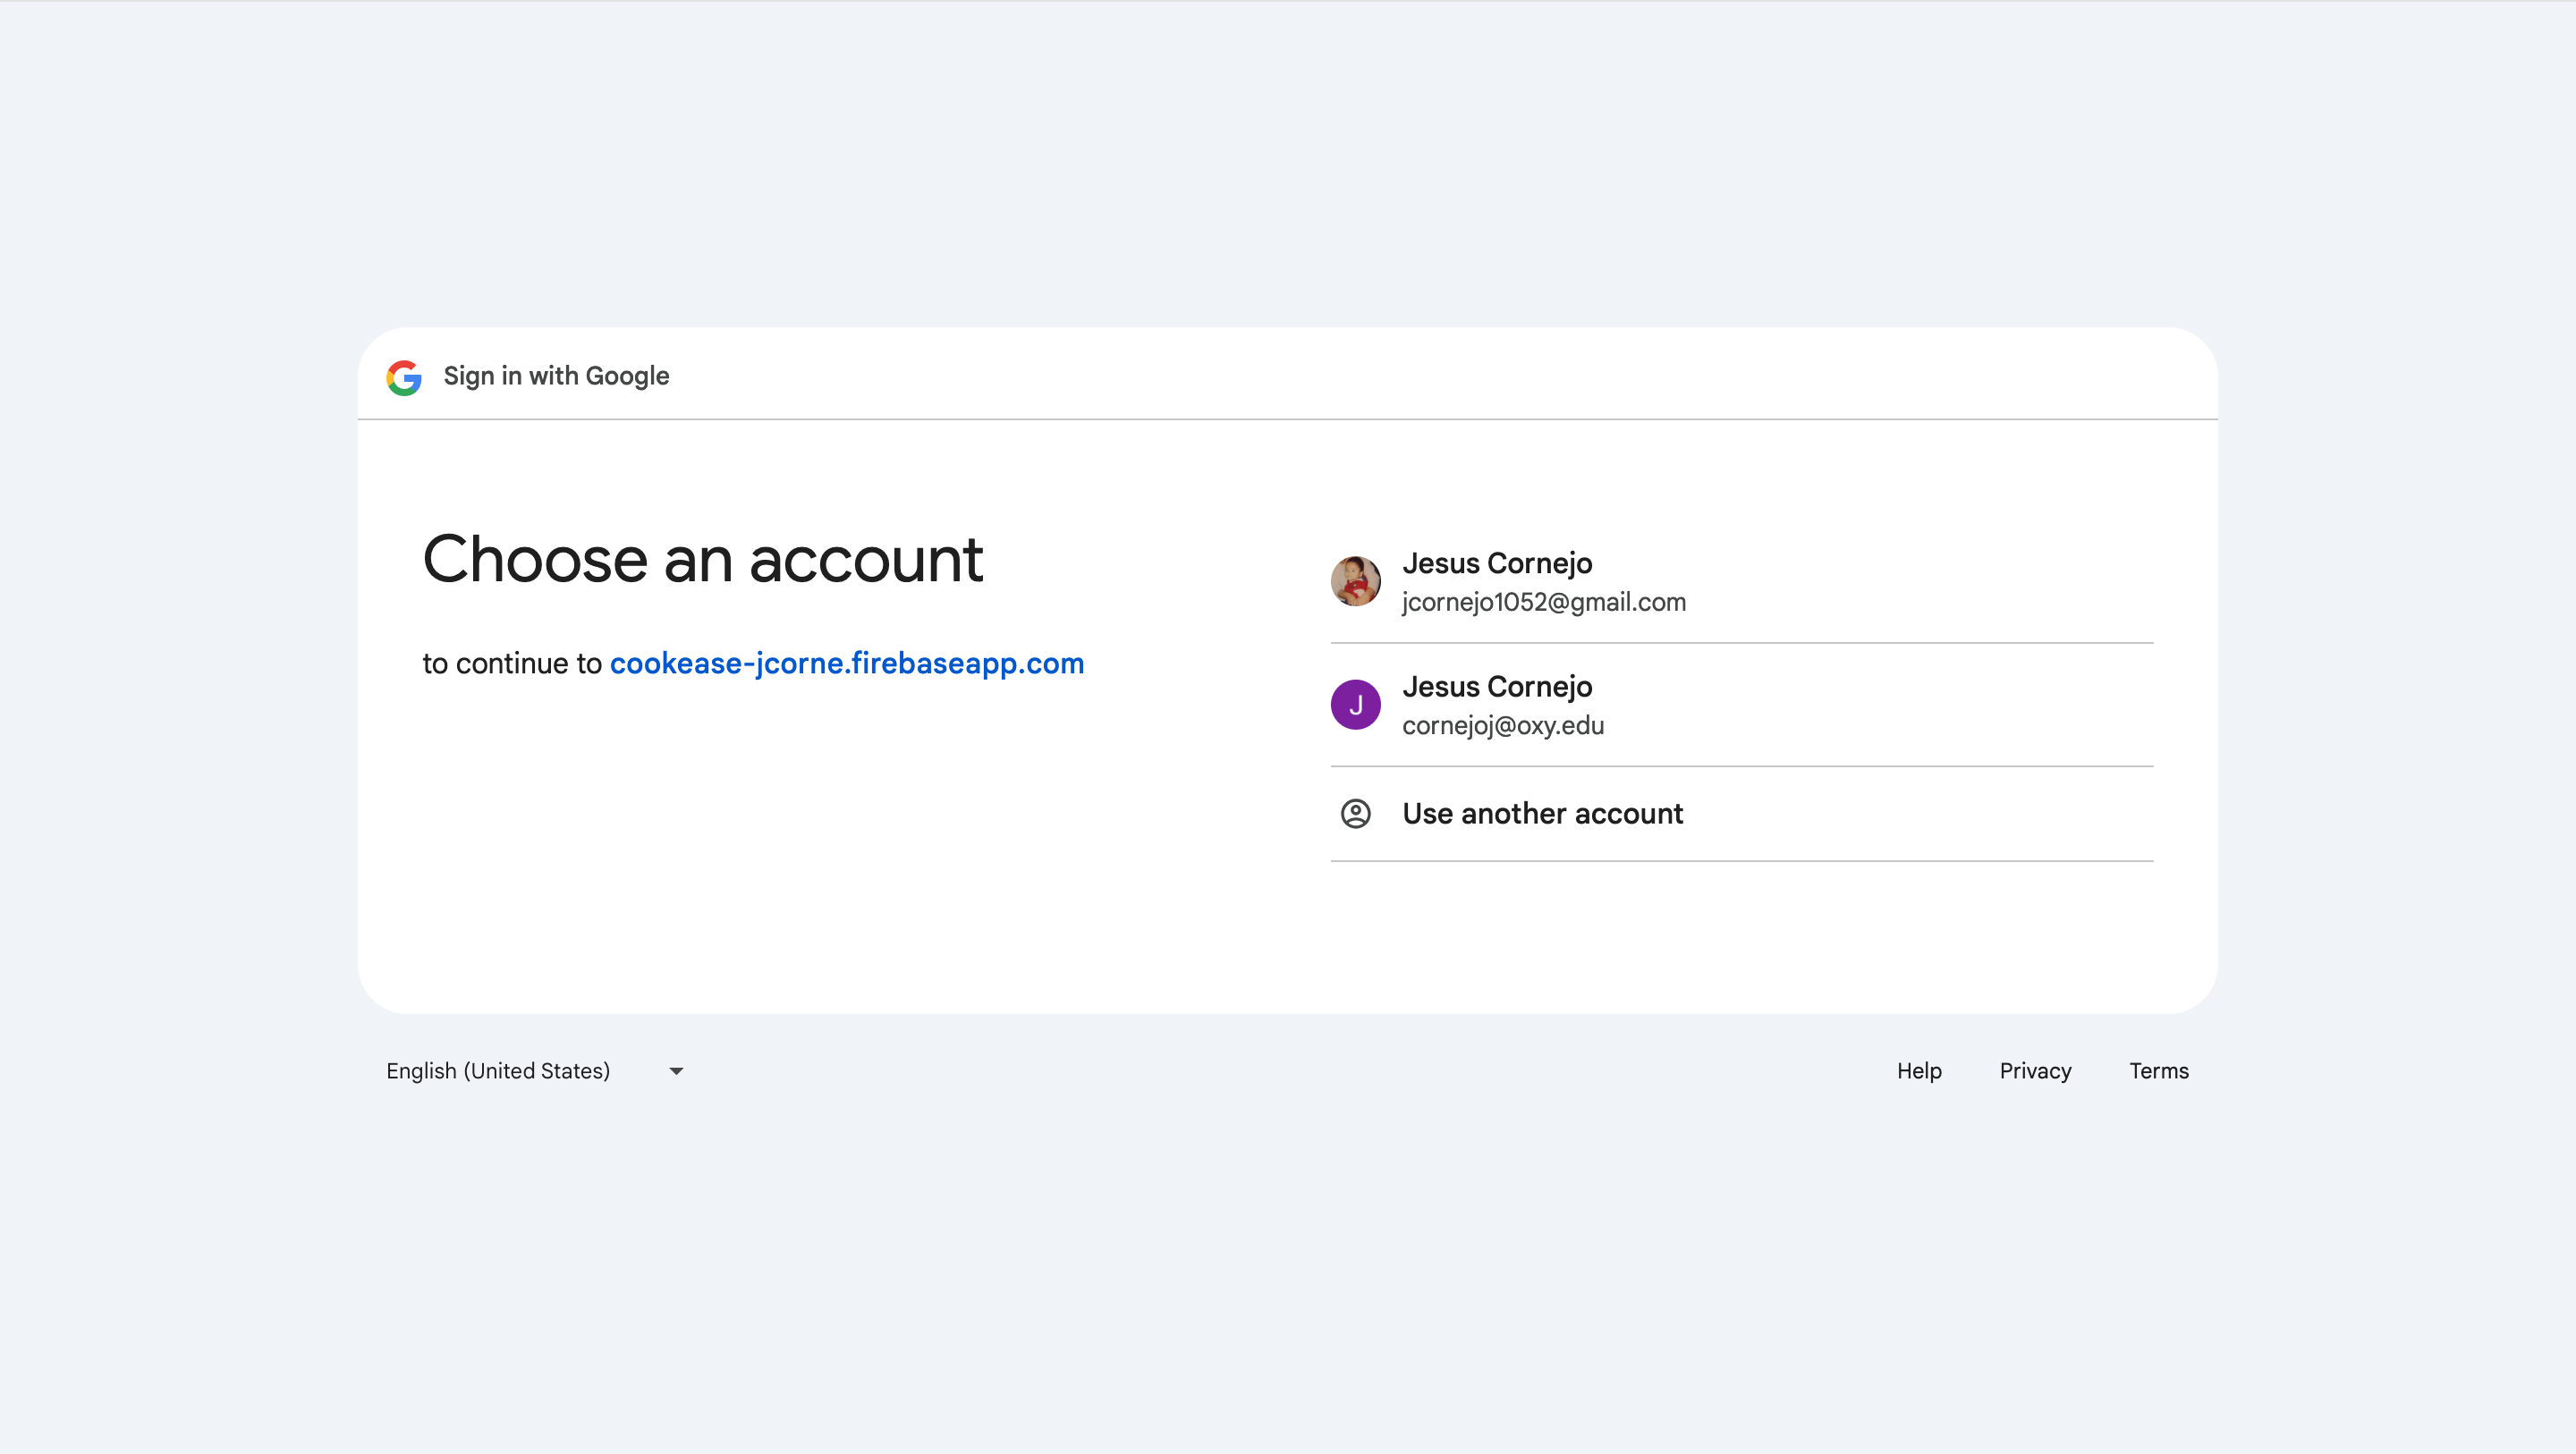
\includegraphics[width=0.5\textwidth]{images/GoogleSignIn.png}
\centering
\end{figure} 
Its features reflect both the technical capabilities of modern web development and the practical needs of its users. By focusing on beginner-friendly design, inventory integration, and guided cooking, CookEase bridges the gaps in existing solutions, offering users an accessible and impactful way to embrace cooking as an enjoyable and sustainable habit.

\section{Methods}
The CookEase project aims to create a comprehensive web application that integrates modern web development technologies and user-centered design principles to address the needs of beginner cooks. This section describes the technical methodologies, algorithms, and system design decisions that contribute to the development of CookEase, detailing how they incorporate insights from prior research and user feedback.

\subsection{System Design and Architecture}
CookEase is built using the MERN stack (MongoDB, Express.js, React, and Node.js), a full-stack development framework that ensures scalability, maintainability, and a seamless integration of frontend and backend functionalities. Each component of the MERN stack contributes to specific aspects of the application:

\textbf{MongoDB} manages user data, such as kitchen inventory, dietary preferences, and meal schedules. Its NoSQL structure enables flexibility, allowing the system to adapt to diverse user inputs and complex relationships between recipes and ingredients.

\textbf{Express.js} serves as the backend framework, handling API requests, user authentication, and data routing between the frontend and the database.

\textbf{React} powers the frontend, providing an interactive user interface with modular components, such as the recipe list, inventory manager, and Cook-Along guide. React's virtual DOM ensures that only the necessary elements are updated, improving performance and user experience.

\textbf{Node.js} supports asynchronous operations on the server side, enabling efficient handling of concurrent API requests and database queries.
\begin{figure}[h!]
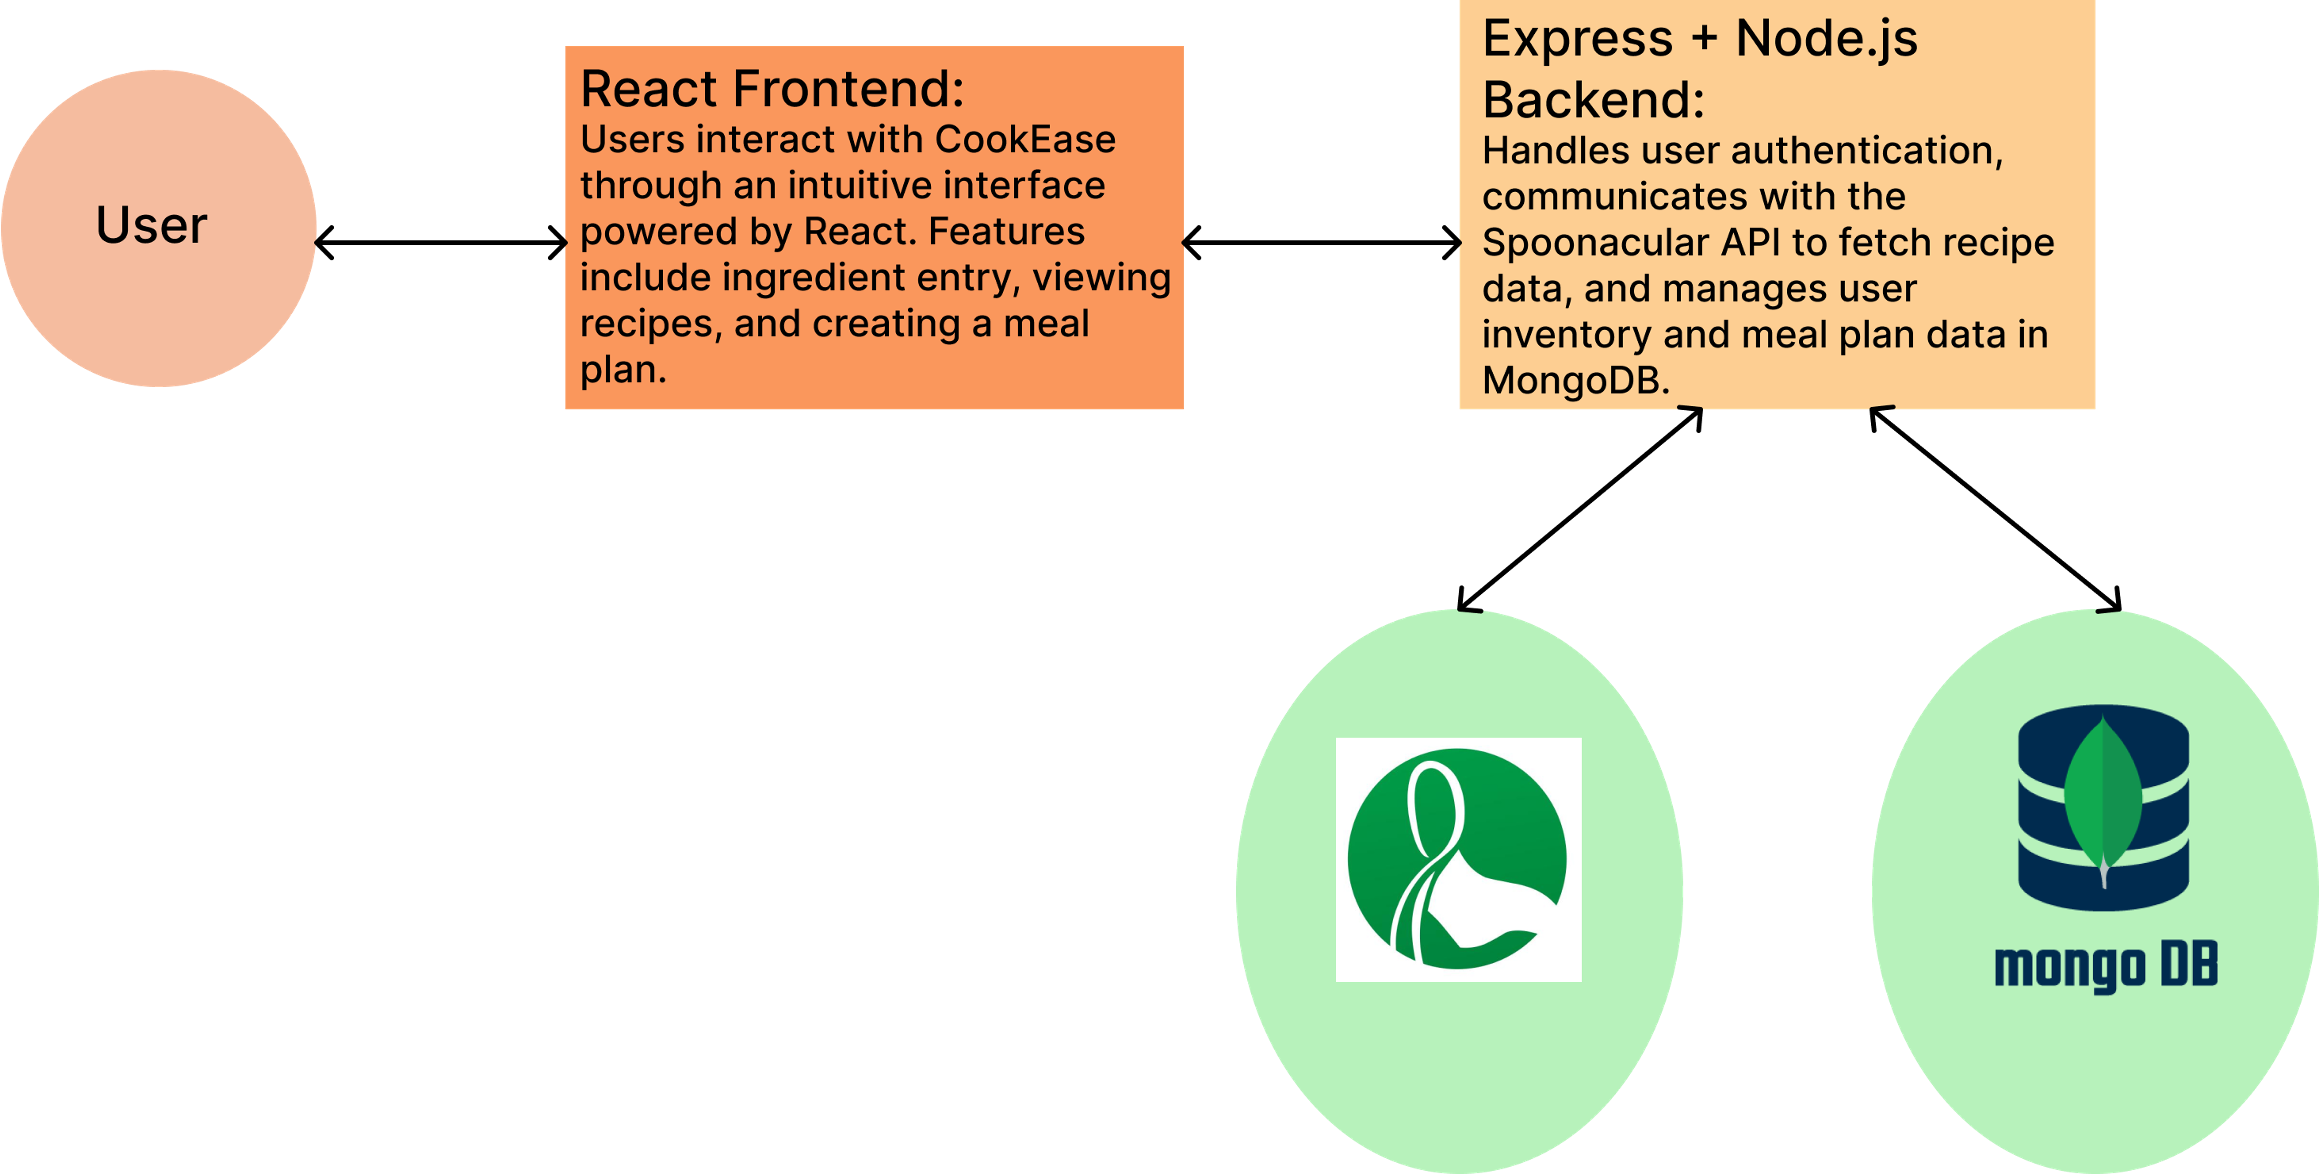
\includegraphics[width=0.5\textwidth]{images/CodeArcDiagram.png}
\centering
\end{figure} 

\subsection{Algorithmic Approaches}
After signing and registering, users will have full access to every component of the CookEase web application. Although CookEase does not employ machine learning, it uses several algorithmic techniques to enhance functionality and user experience:

\subsubsection{Ingredient Matching:}
CookEase incorporates an ingredient-matching algorithm to filter recipes from the Spoonacular API. This algorithm matches user-provided ingredients with those required in recipes, prioritizing recipes that maximize ingredient usage while minimizing additional purchases.

\begin{figure}[h!]
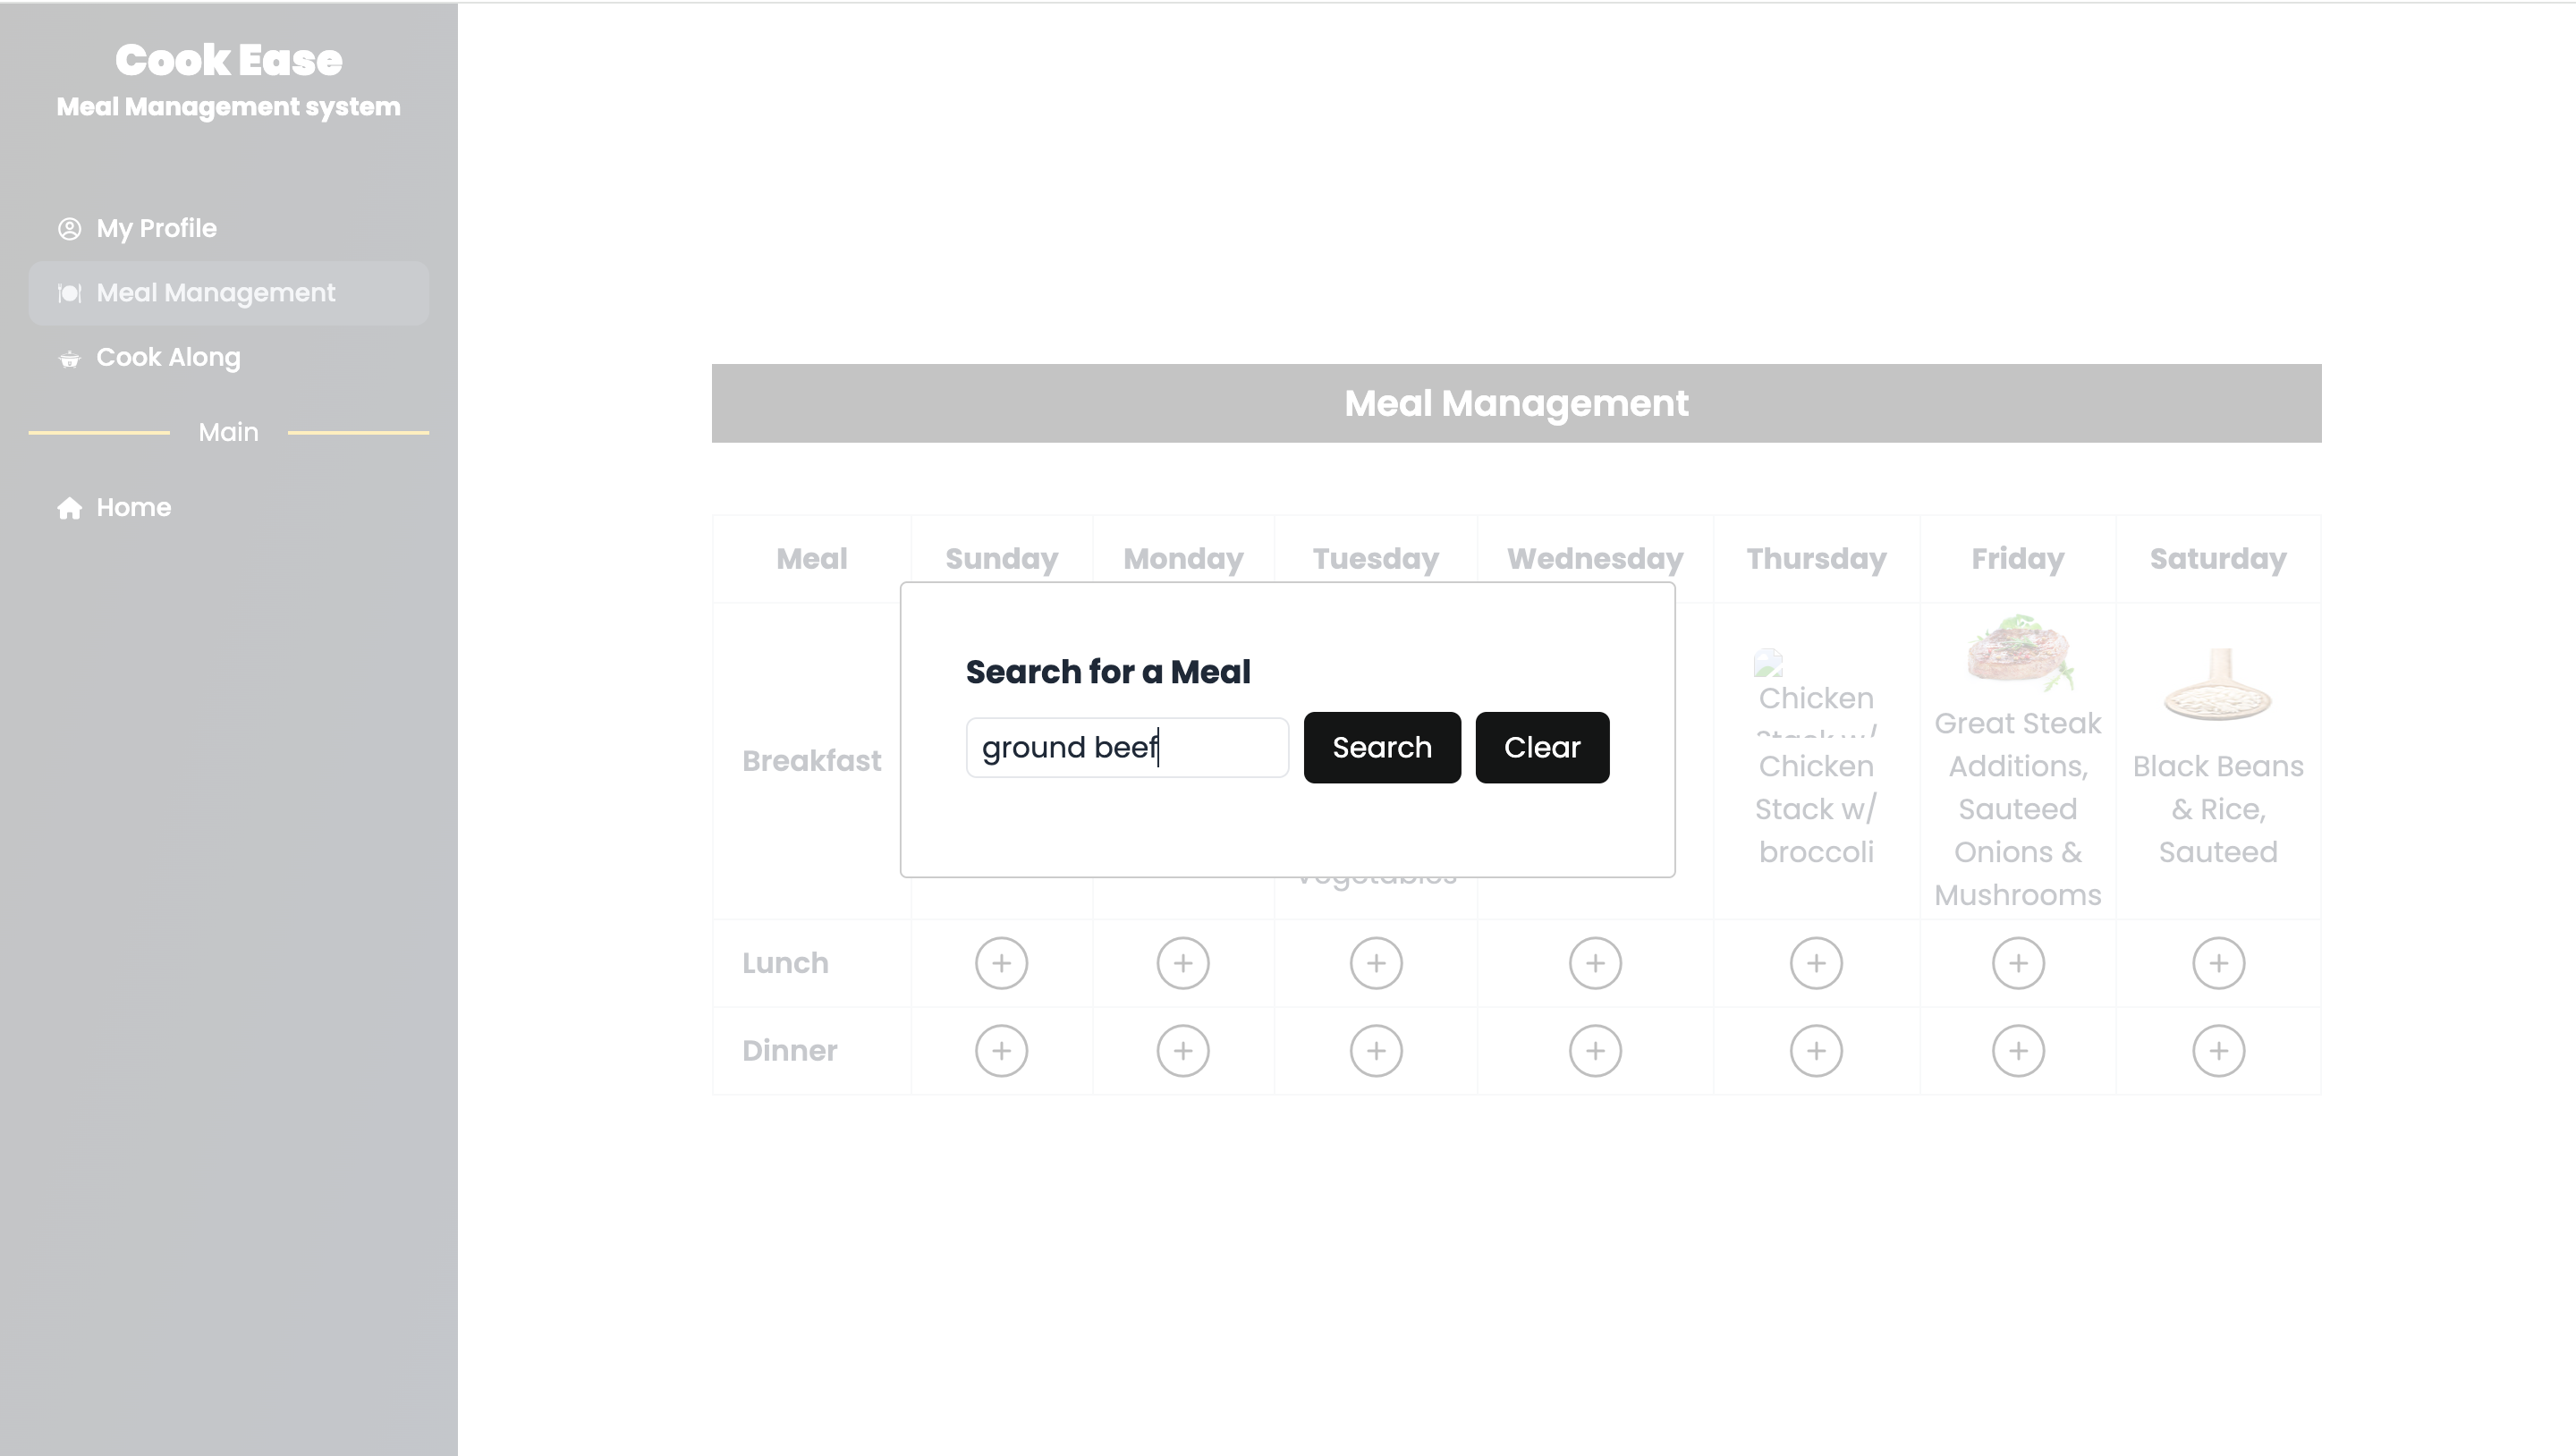
\includegraphics[width=0.5\textwidth]{images/Search.png}
\centering
\end{figure}
\begin{figure}[h!]
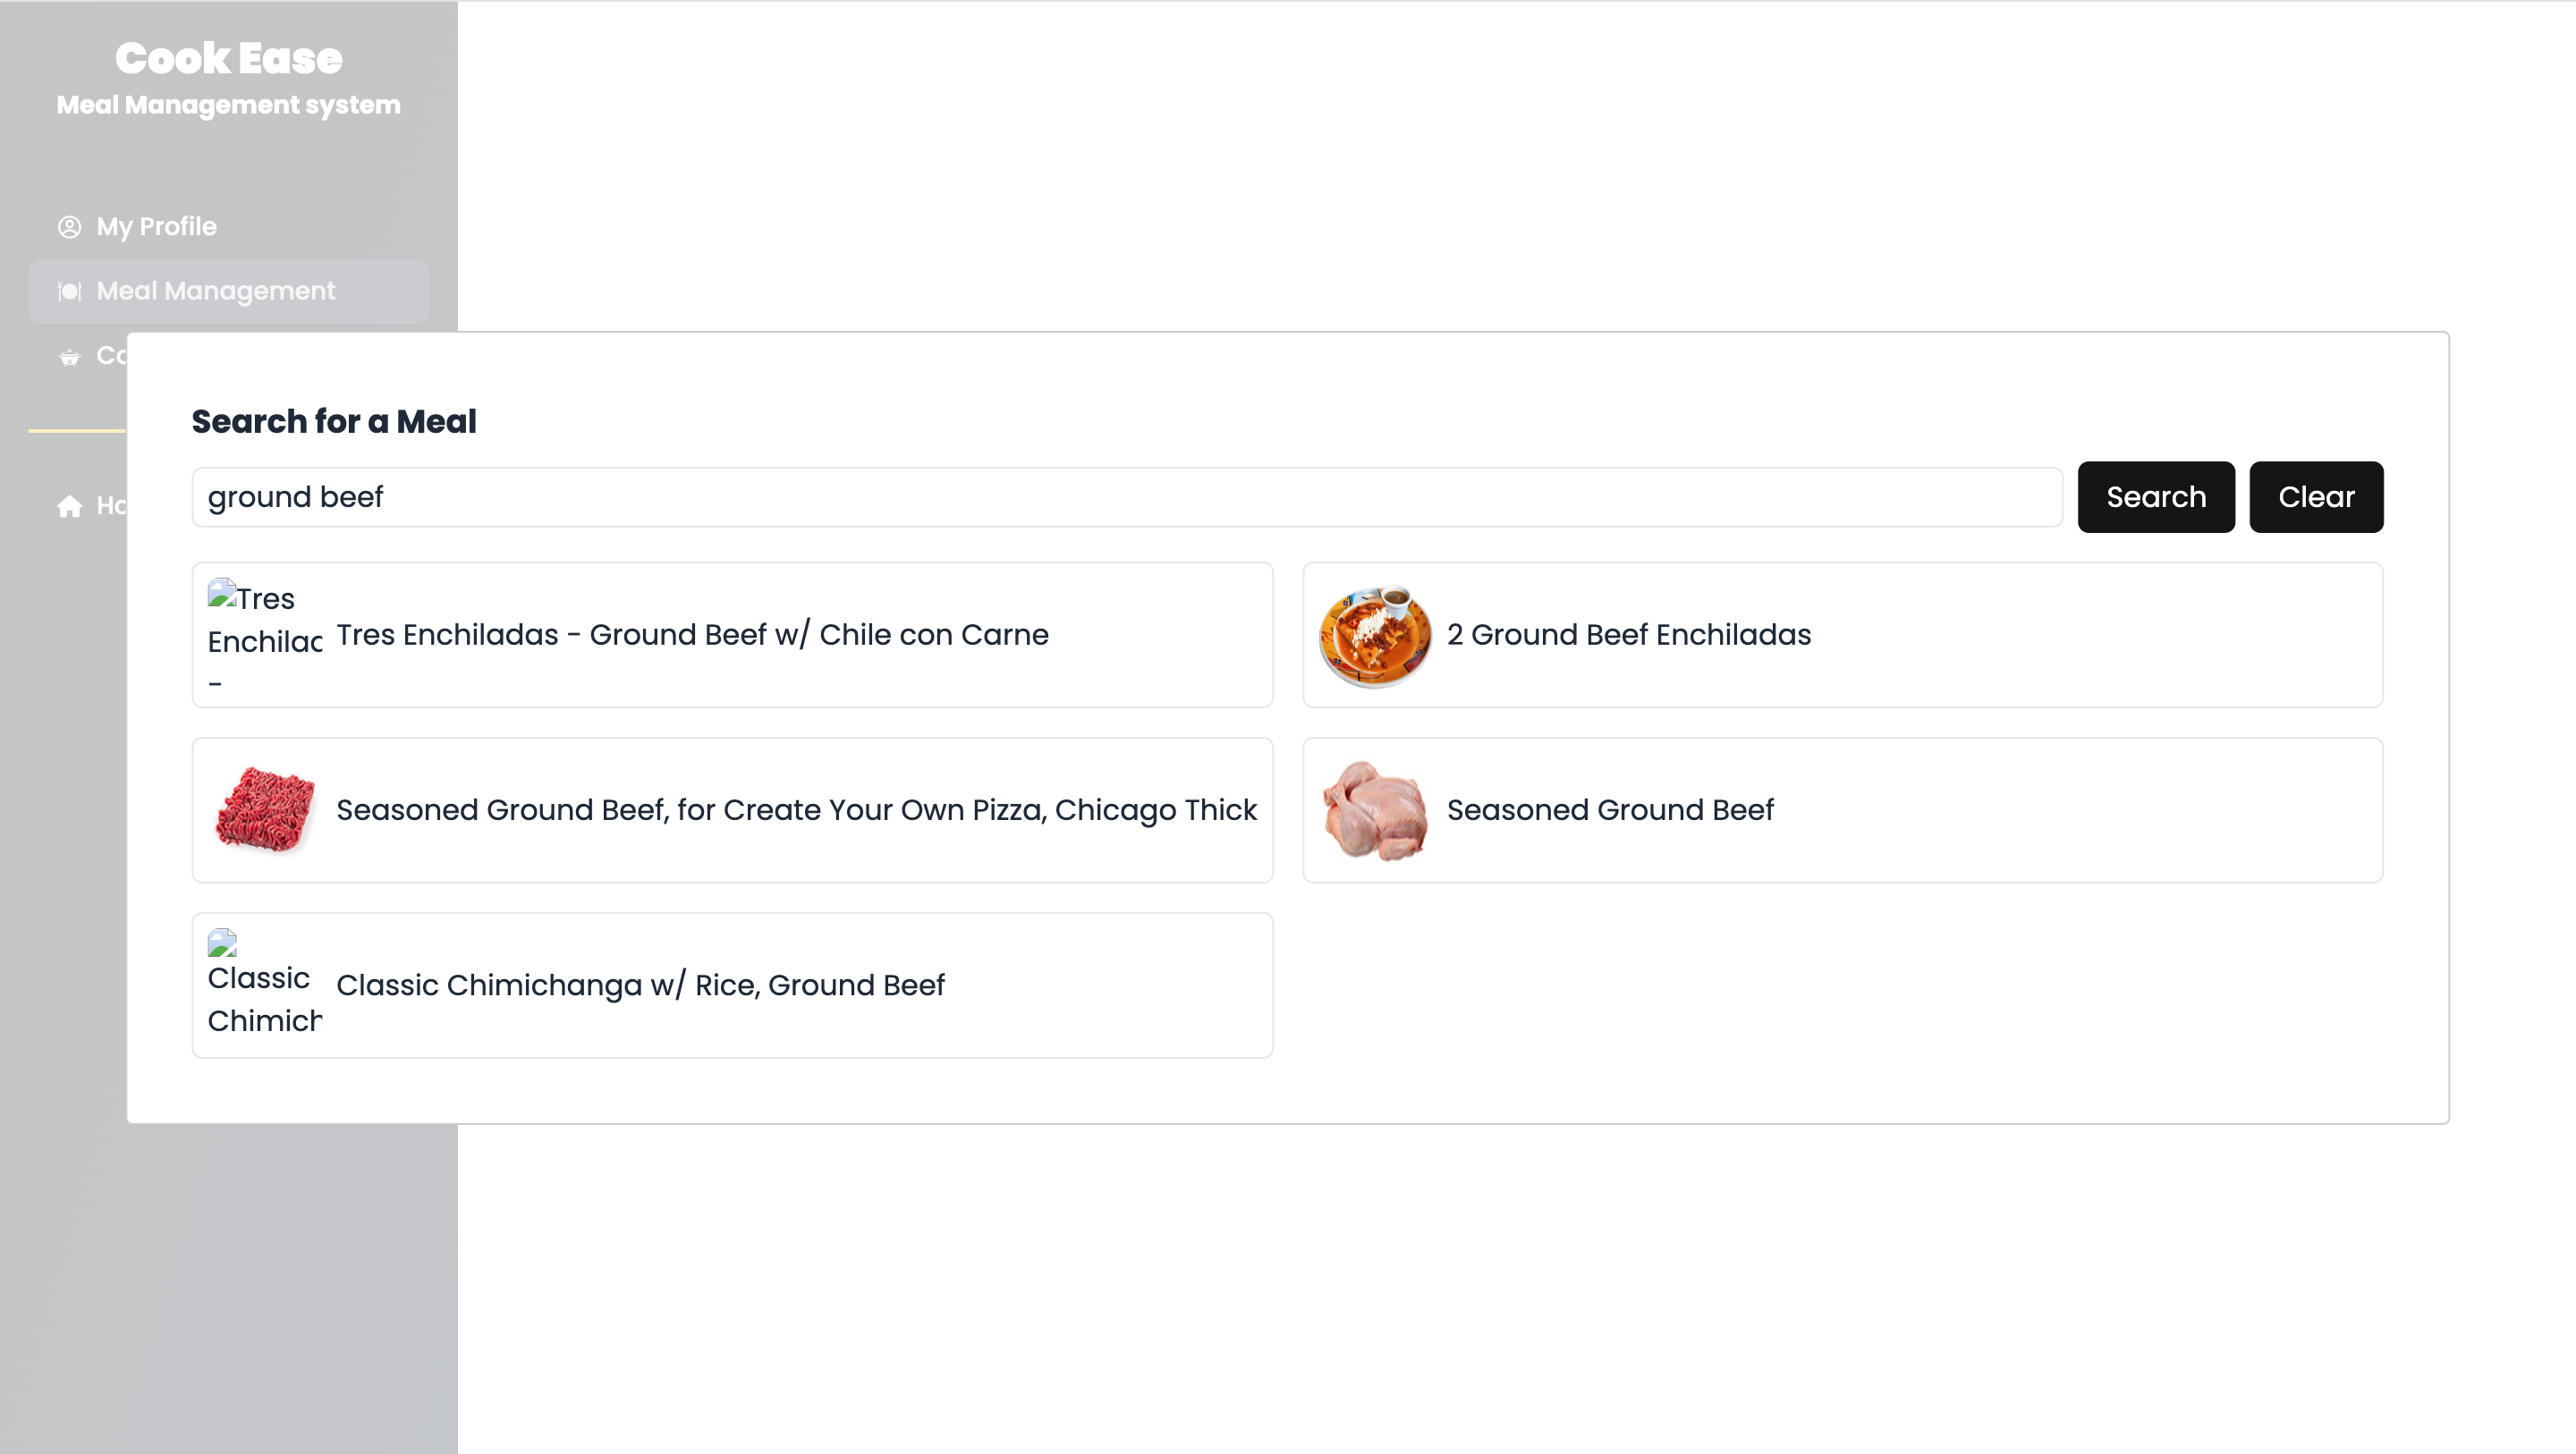
\includegraphics[width=0.5\textwidth]{images/SearchResults.png}
\centering
\end{figure} 

\subsubsection{Inventory Tracking:}
A simple counting algorithm is used to track the availability of ingredients in the user’s kitchen inventory. (This feature was used in a previous version of CookEase, but after user testing and reviews I decided not to focus on this feature as much going forward.)

\subsubsection{Meal Scheduling:}
The meal scheduling algorithm ensures that users can plan meals without overlapping times or conflicting schedules. It assigns recipes to specific dates and times based on user input.


\subsection{API Integration and Data Flow}
CookEase relies on the Spoonacular API for recipe generation and culinary data. The integration involves the following steps:

API Request Handling: The frontend sends user data, such as ingredients and dietary preferences, to the backend via HTTP POST requests. The backend processes these requests and forwards them to the Spoonacular API.
Data Parsing: The raw data received from the API includes a large dataset with recipe details, such as ingredients, instructions, and nutritional information. CookEase parses this data to extract relevant fields, which are then structured for easy display and interaction on the frontend.
Error Handling: To ensure reliability, the system implements robust error-handling mechanisms. These include fallback responses for network failures and alternative suggestions when the API fails to return relevant recipes.
\begin{figure}[h!]
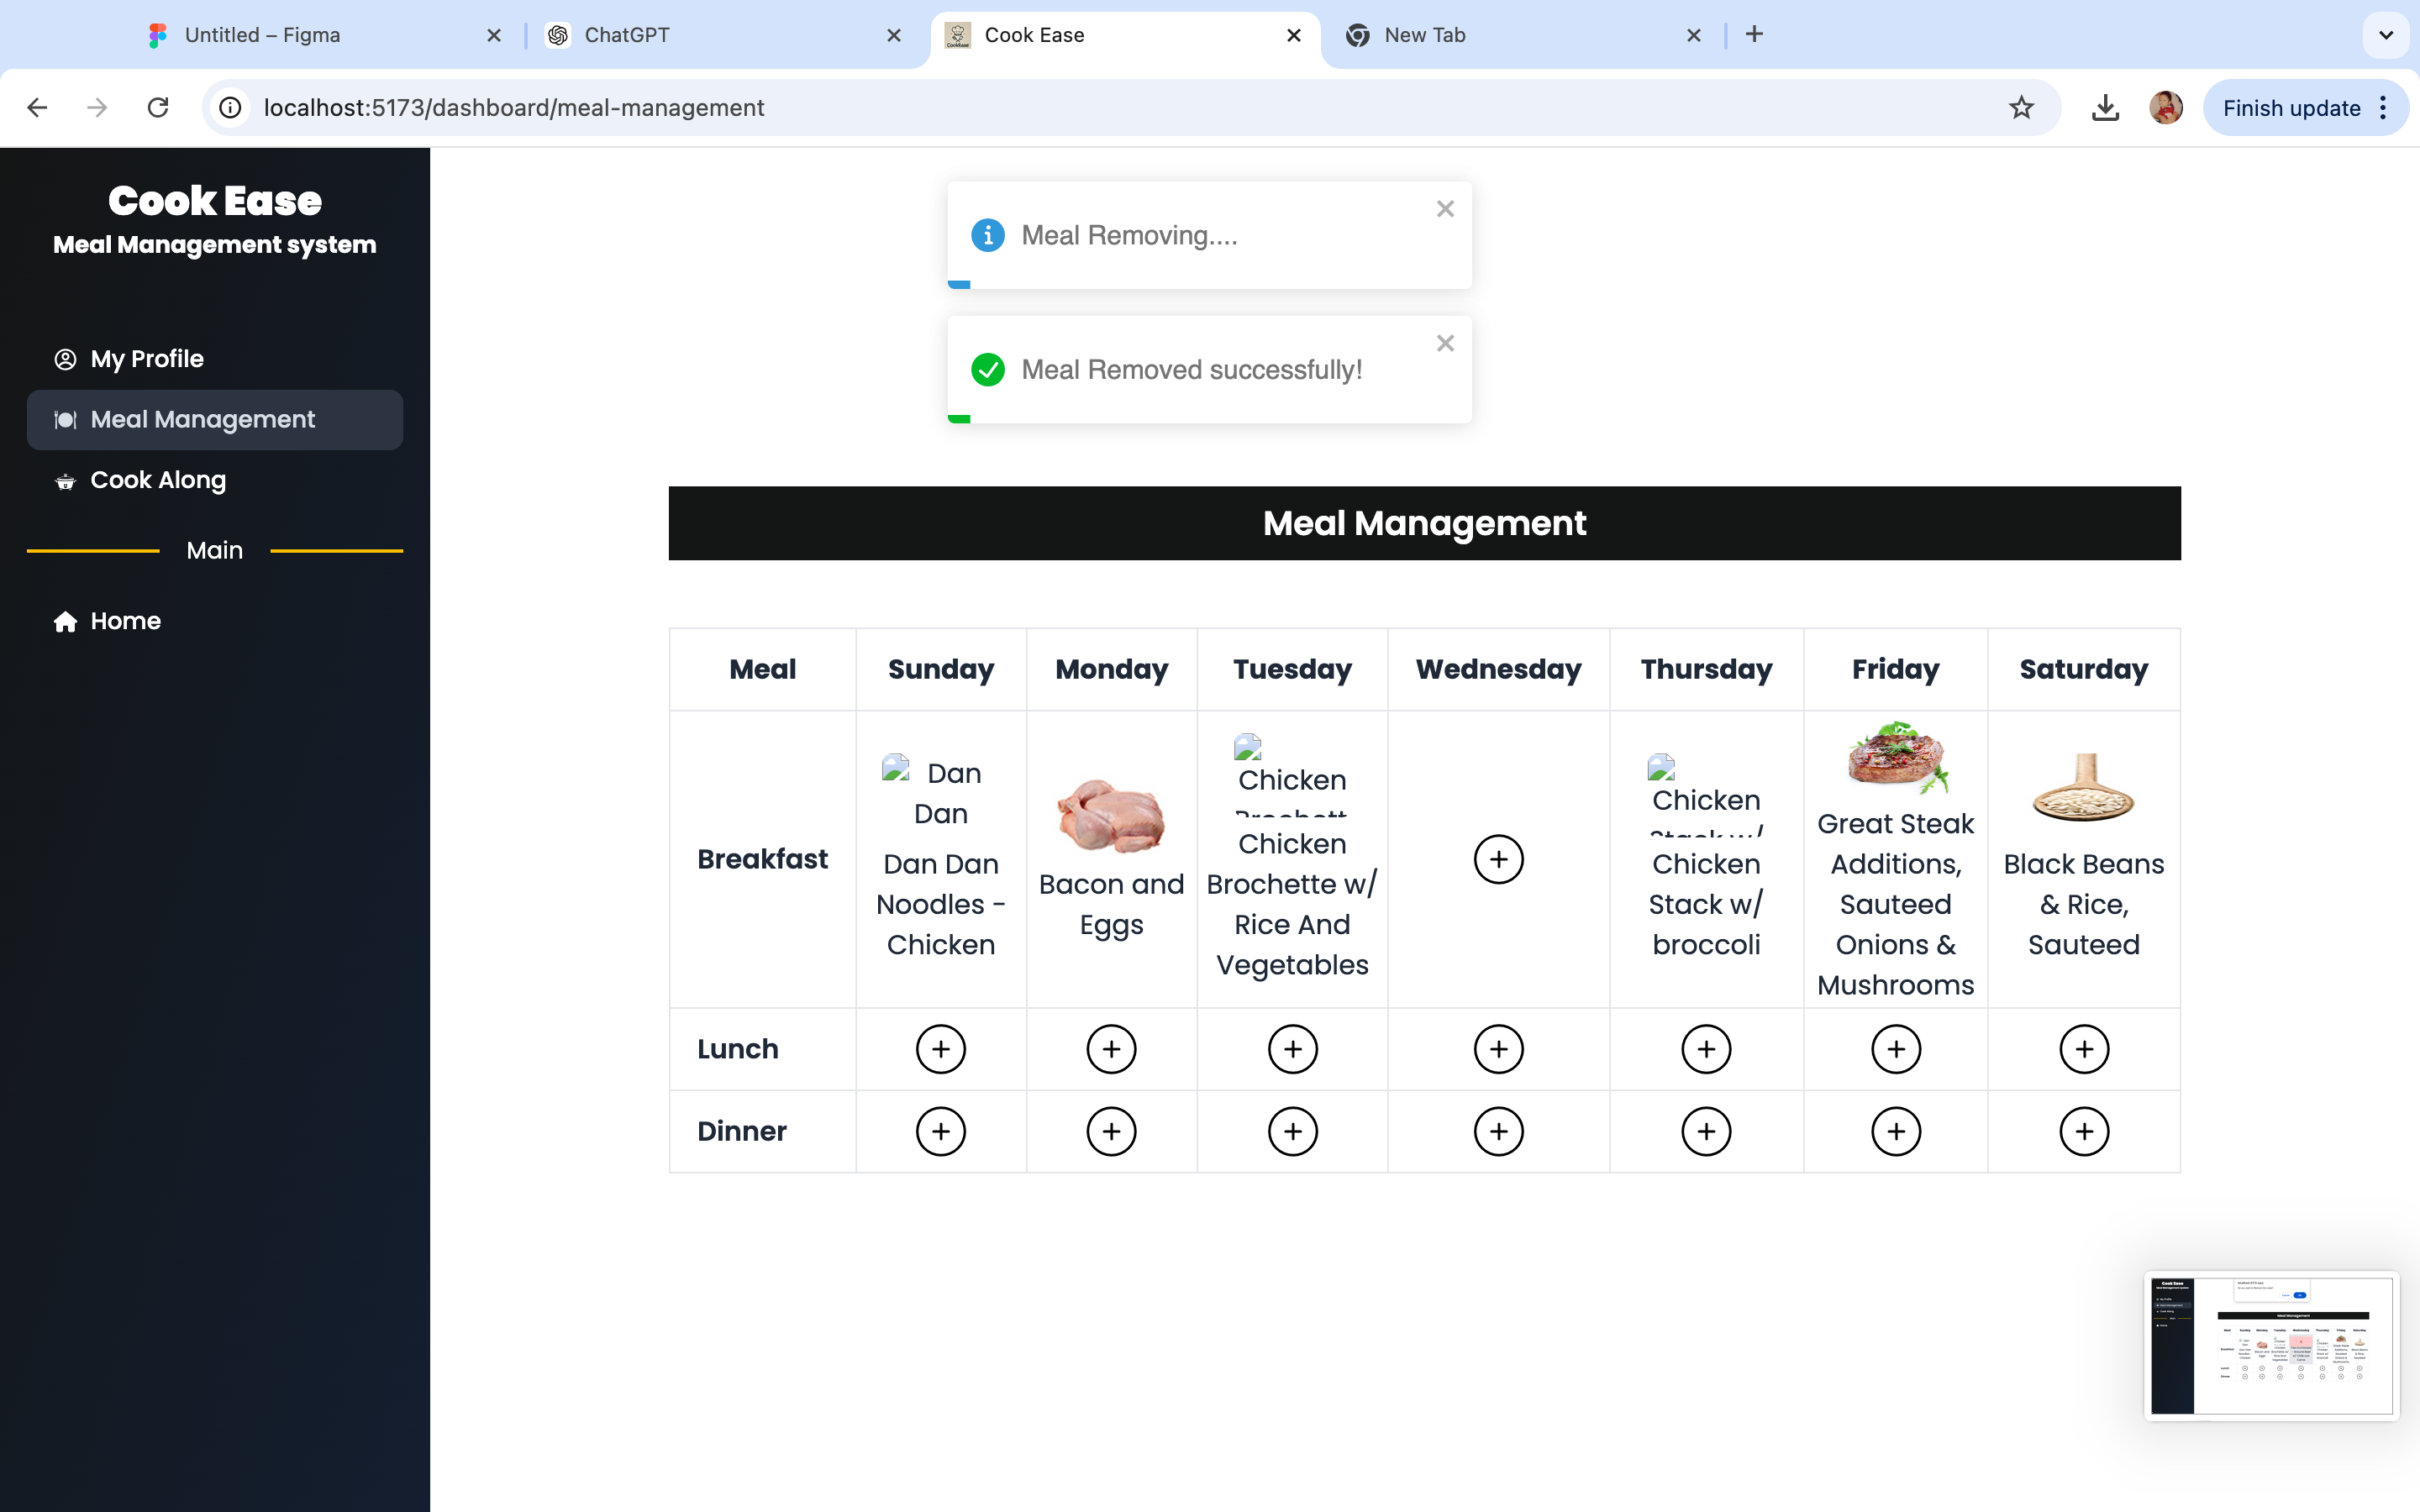
\includegraphics[width=0.5\textwidth]{images/RemovingMeal.png}
\centering
\end{figure} 

\subsection{Feature Implementation}
The primary features of CookEase are implemented with a focus on usability and beginner support:
\begin{itemize}
    \item Recipe Generation: Recipes are generated based on the user's current kitchen inventory and preferences in the search. The ingredient-matching algorithm from Spoonacular API filters the results, ensuring that suggestions align with the user’s available resources. Additionally, recipes are ranked by relevance, with options to substitute missing ingredients. 
    \begin{figure}[h!]
    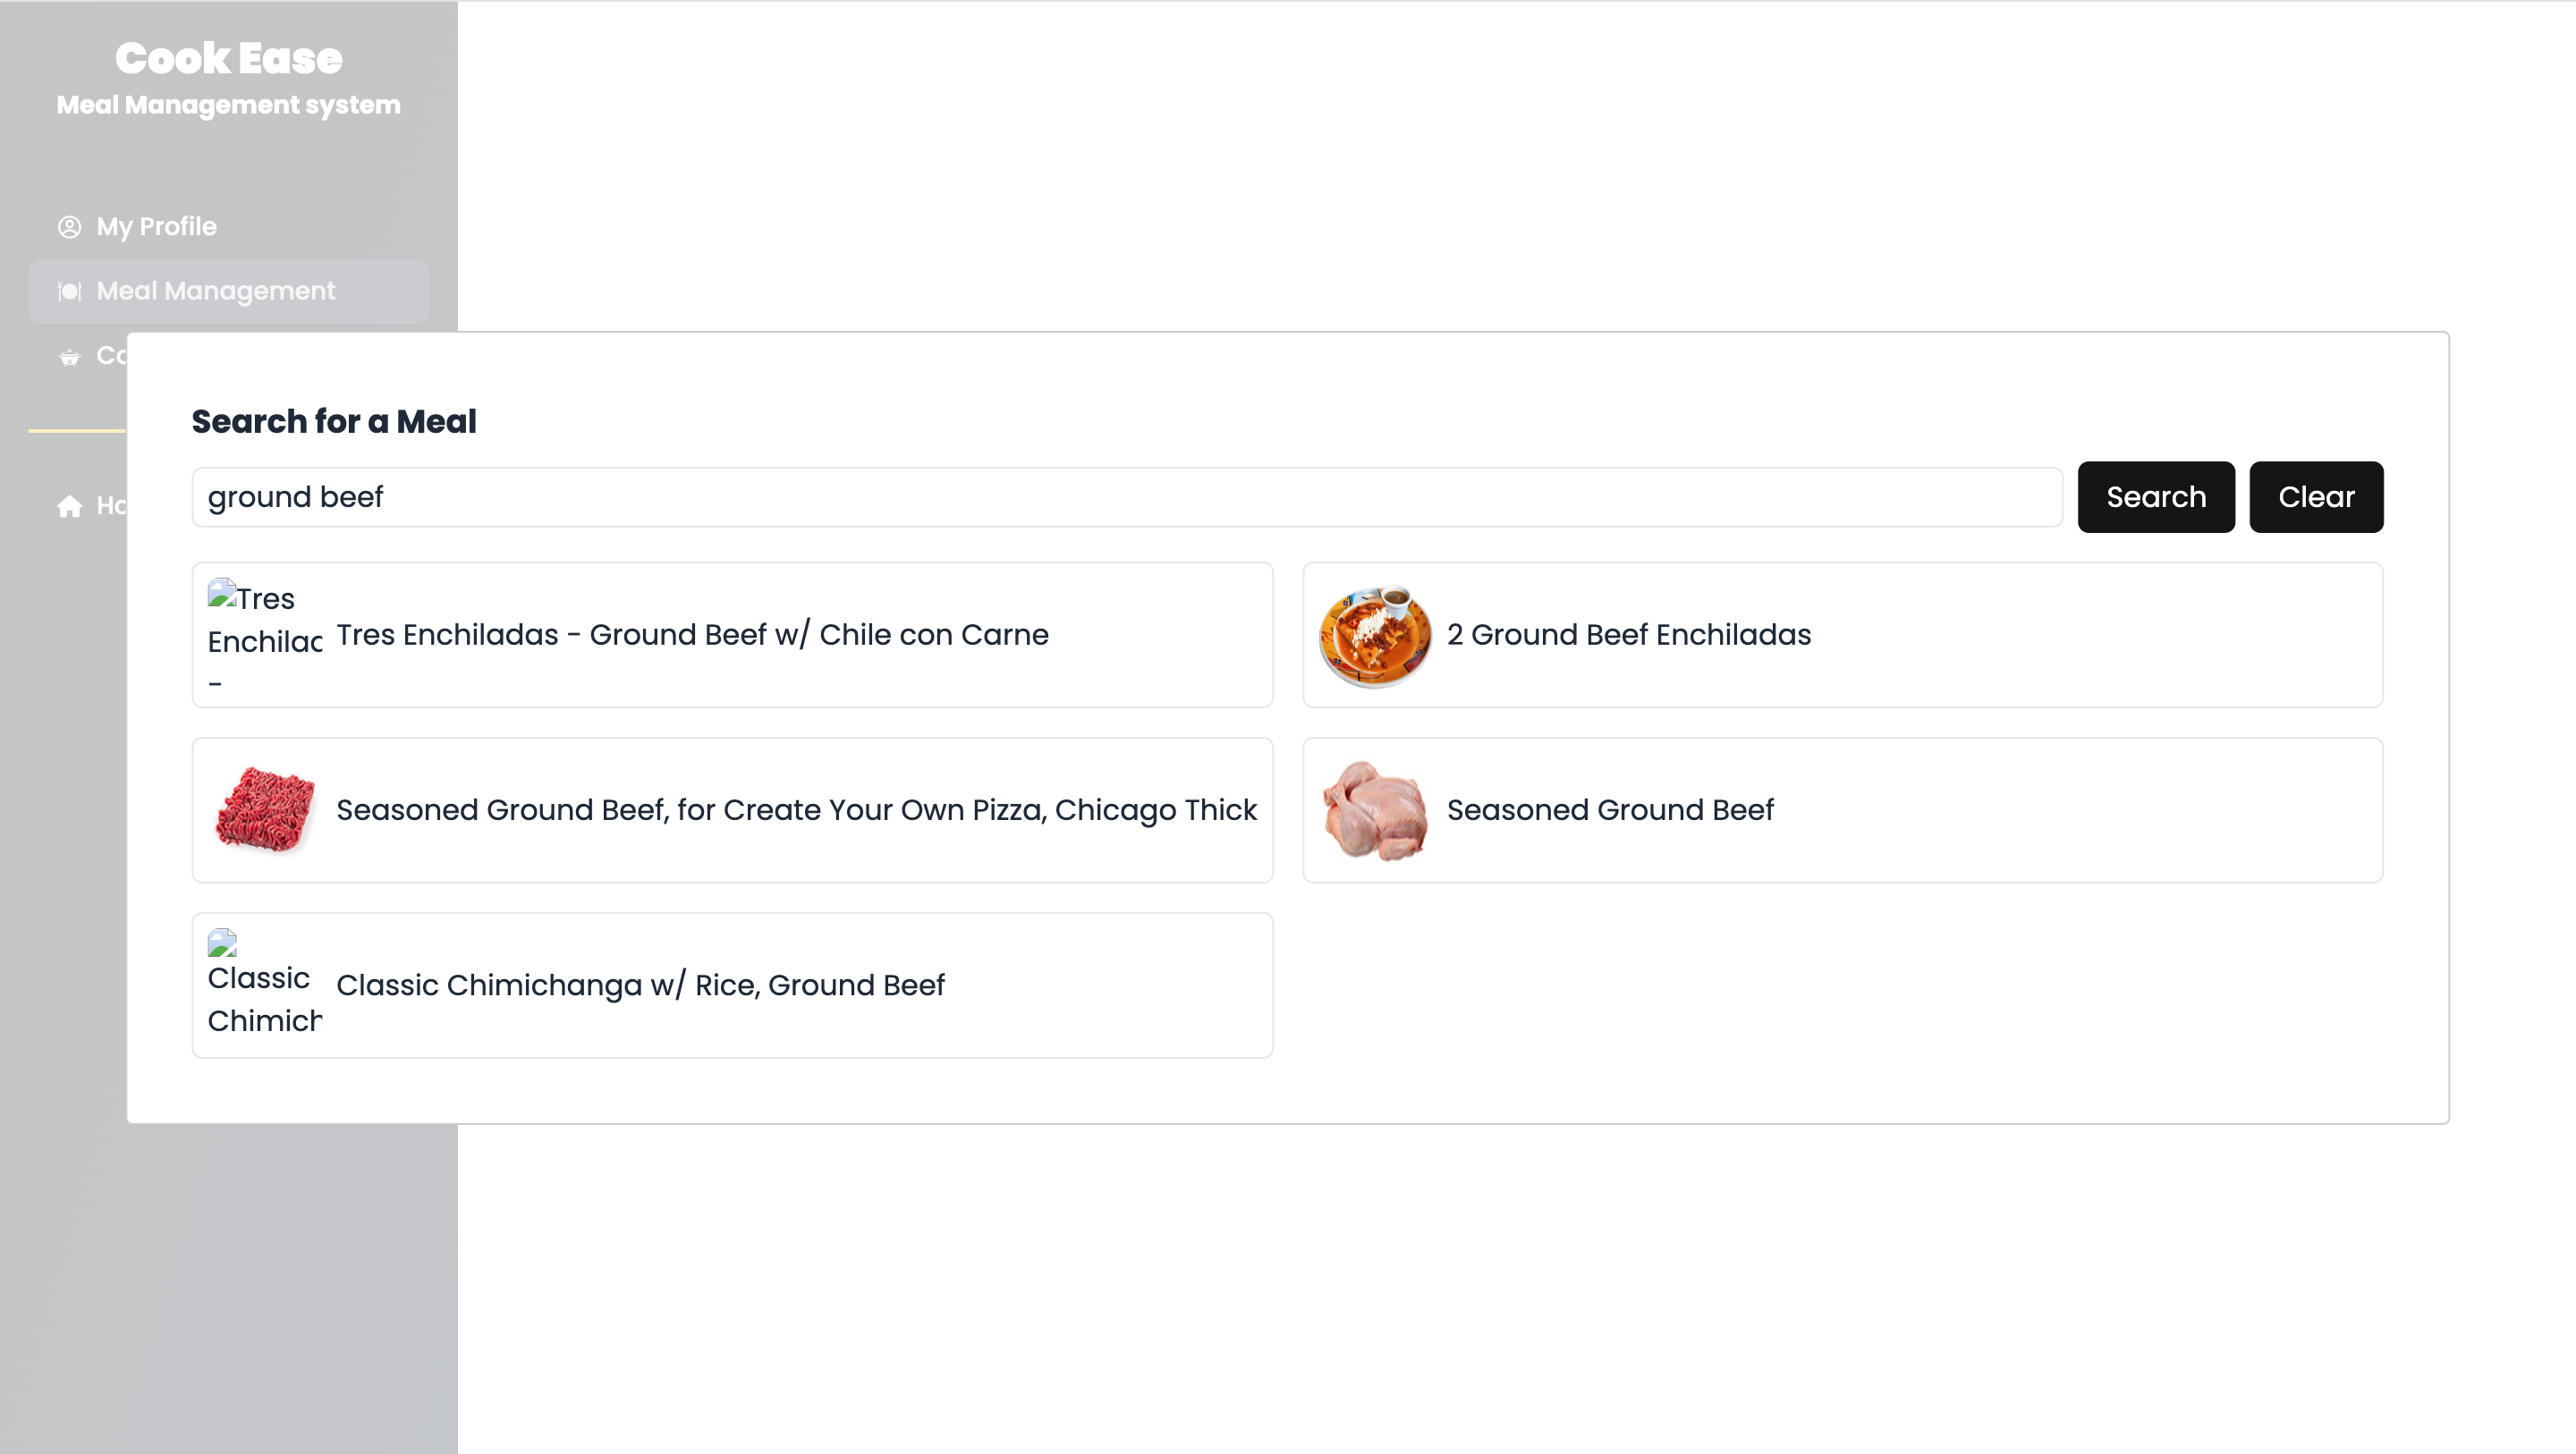
\includegraphics[width=0.5\textwidth]{images/SearchResults.png}
    \centering
    \end{figure} 
    
    \item Cook-Along Guide: This interactive feature breaks recipes into detailed steps with clear instructions. Each step includes guidance on preparation, cooking techniques, and timing. The guide is designed to provide reassurance and support, particularly for users with limited cooking experience. A simple timer is included for users, to help with steps that may require it.
    \begin{figure}[h!]
    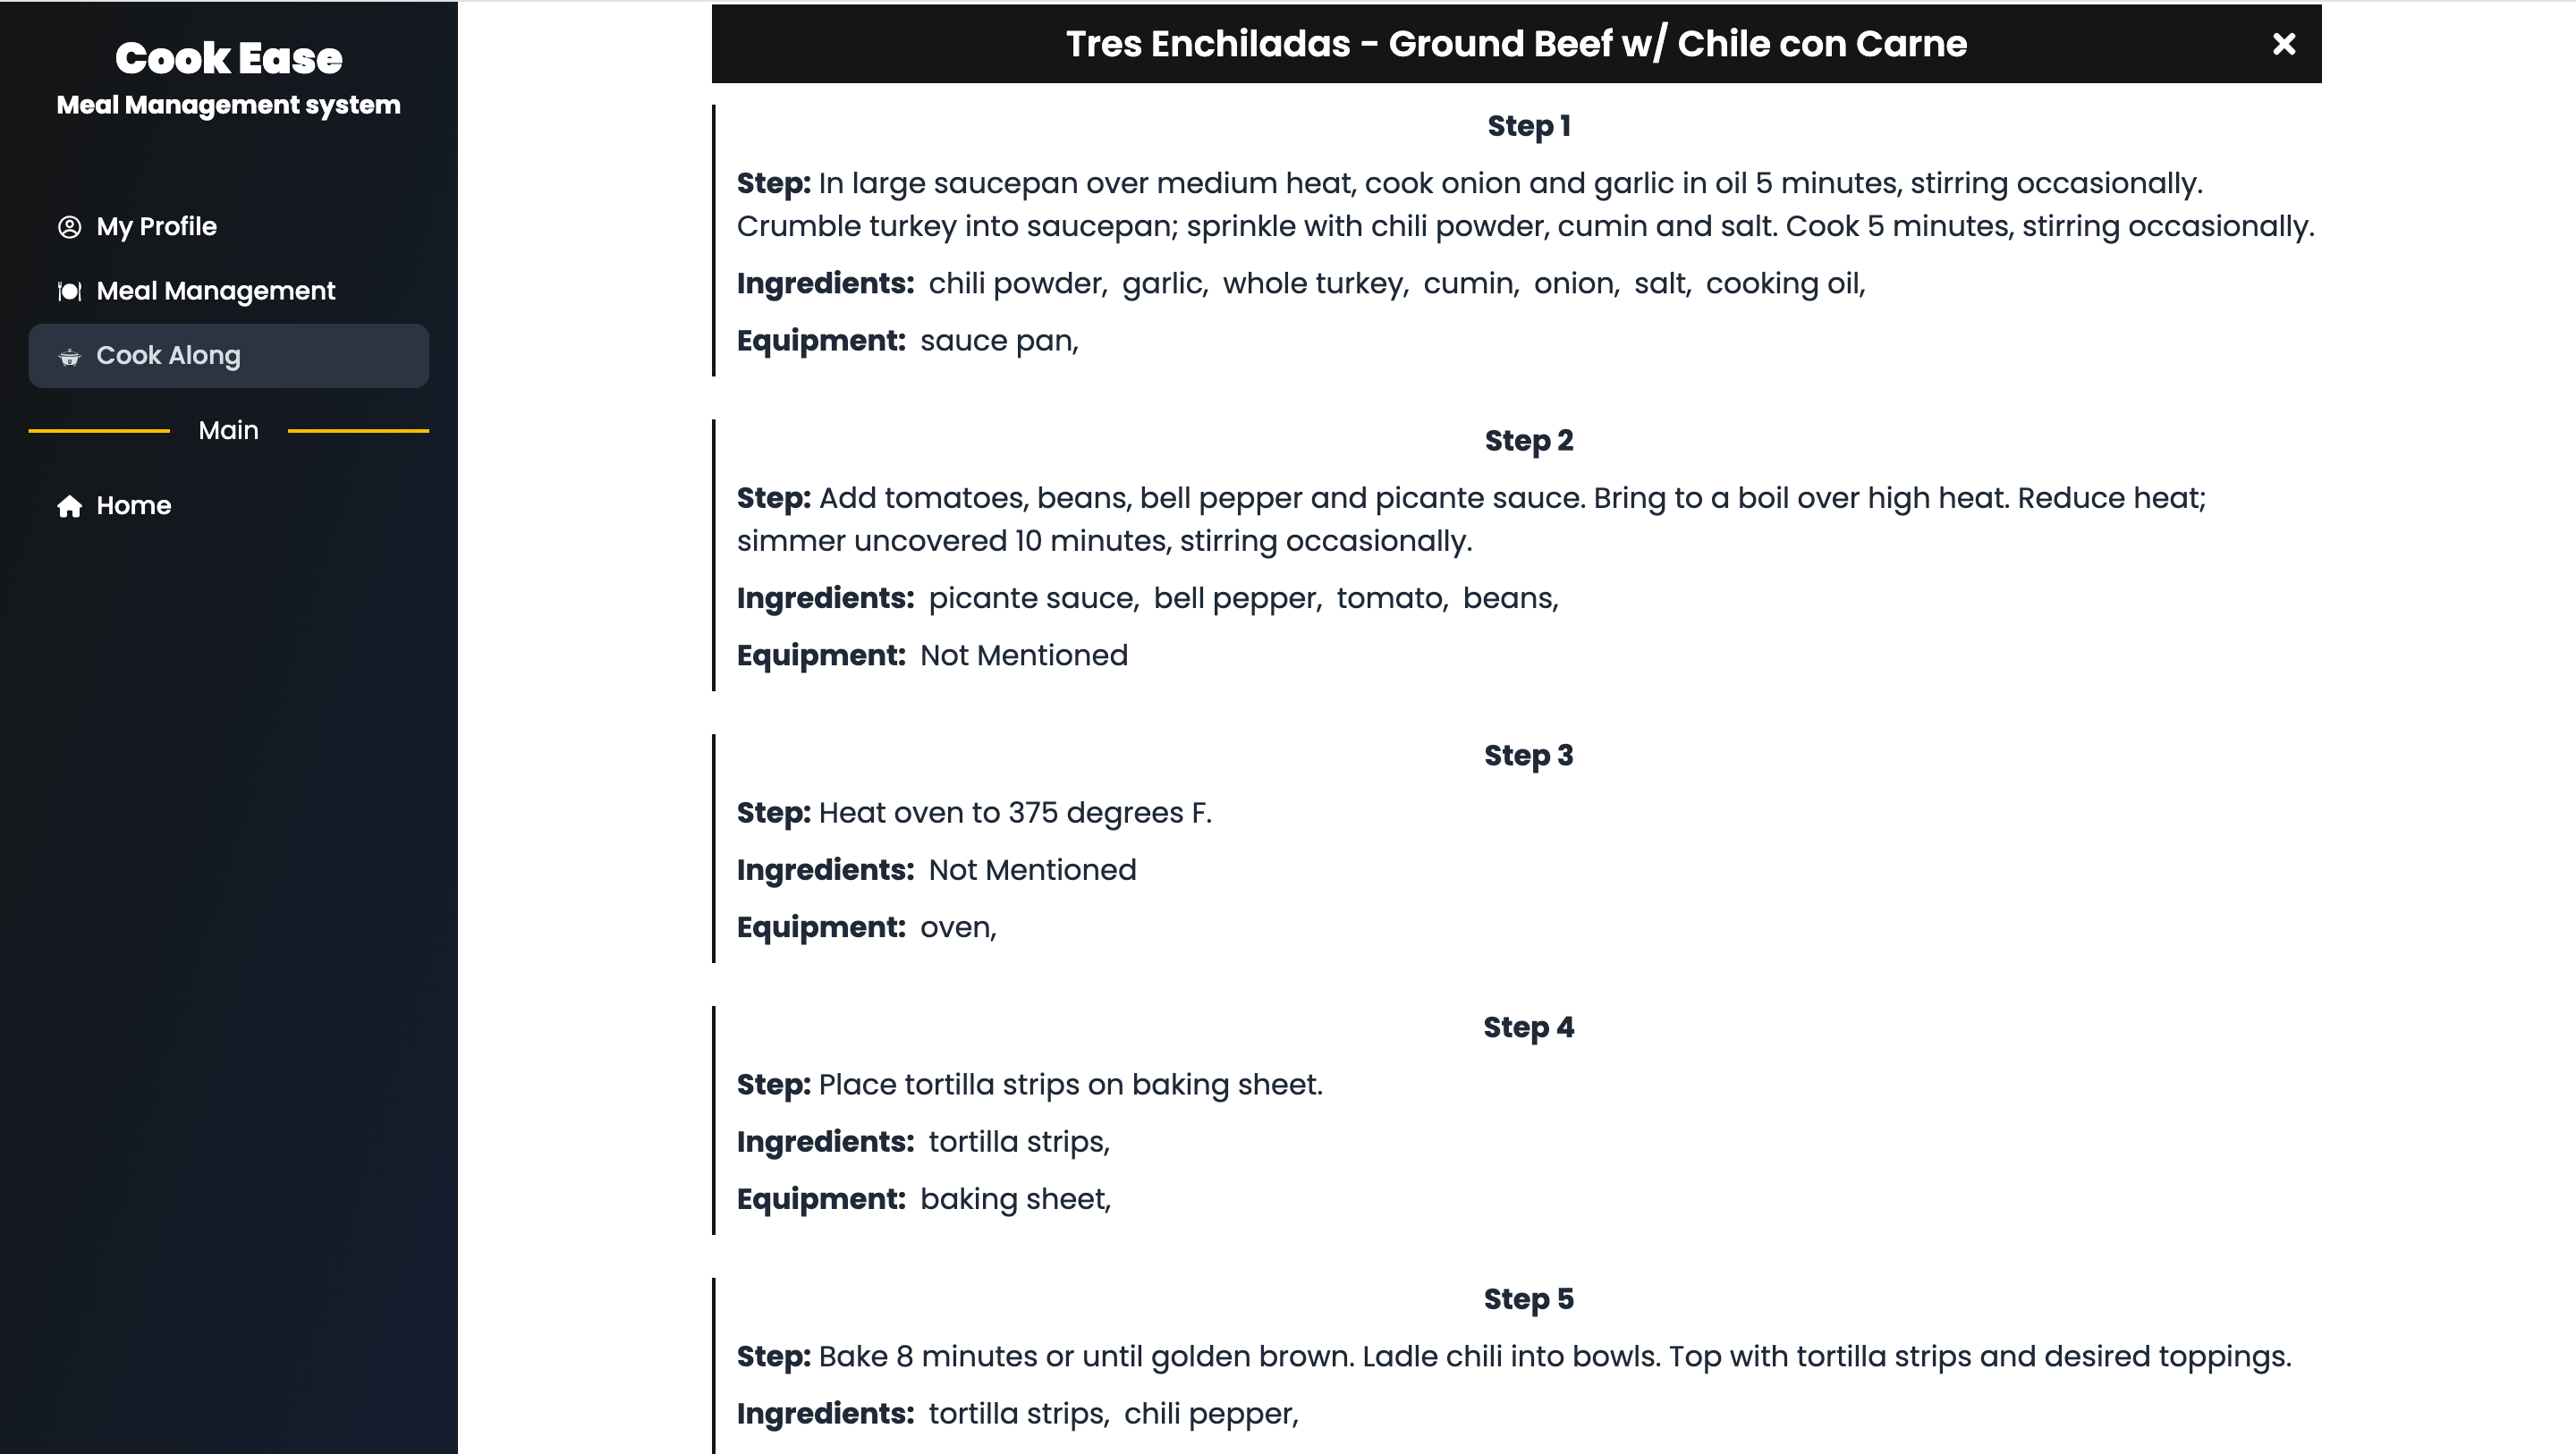
\includegraphics[width=0.5\textwidth]{images/CookAlong.png}
    \centering
    \end{figure}
    \begin{figure}[h!]
    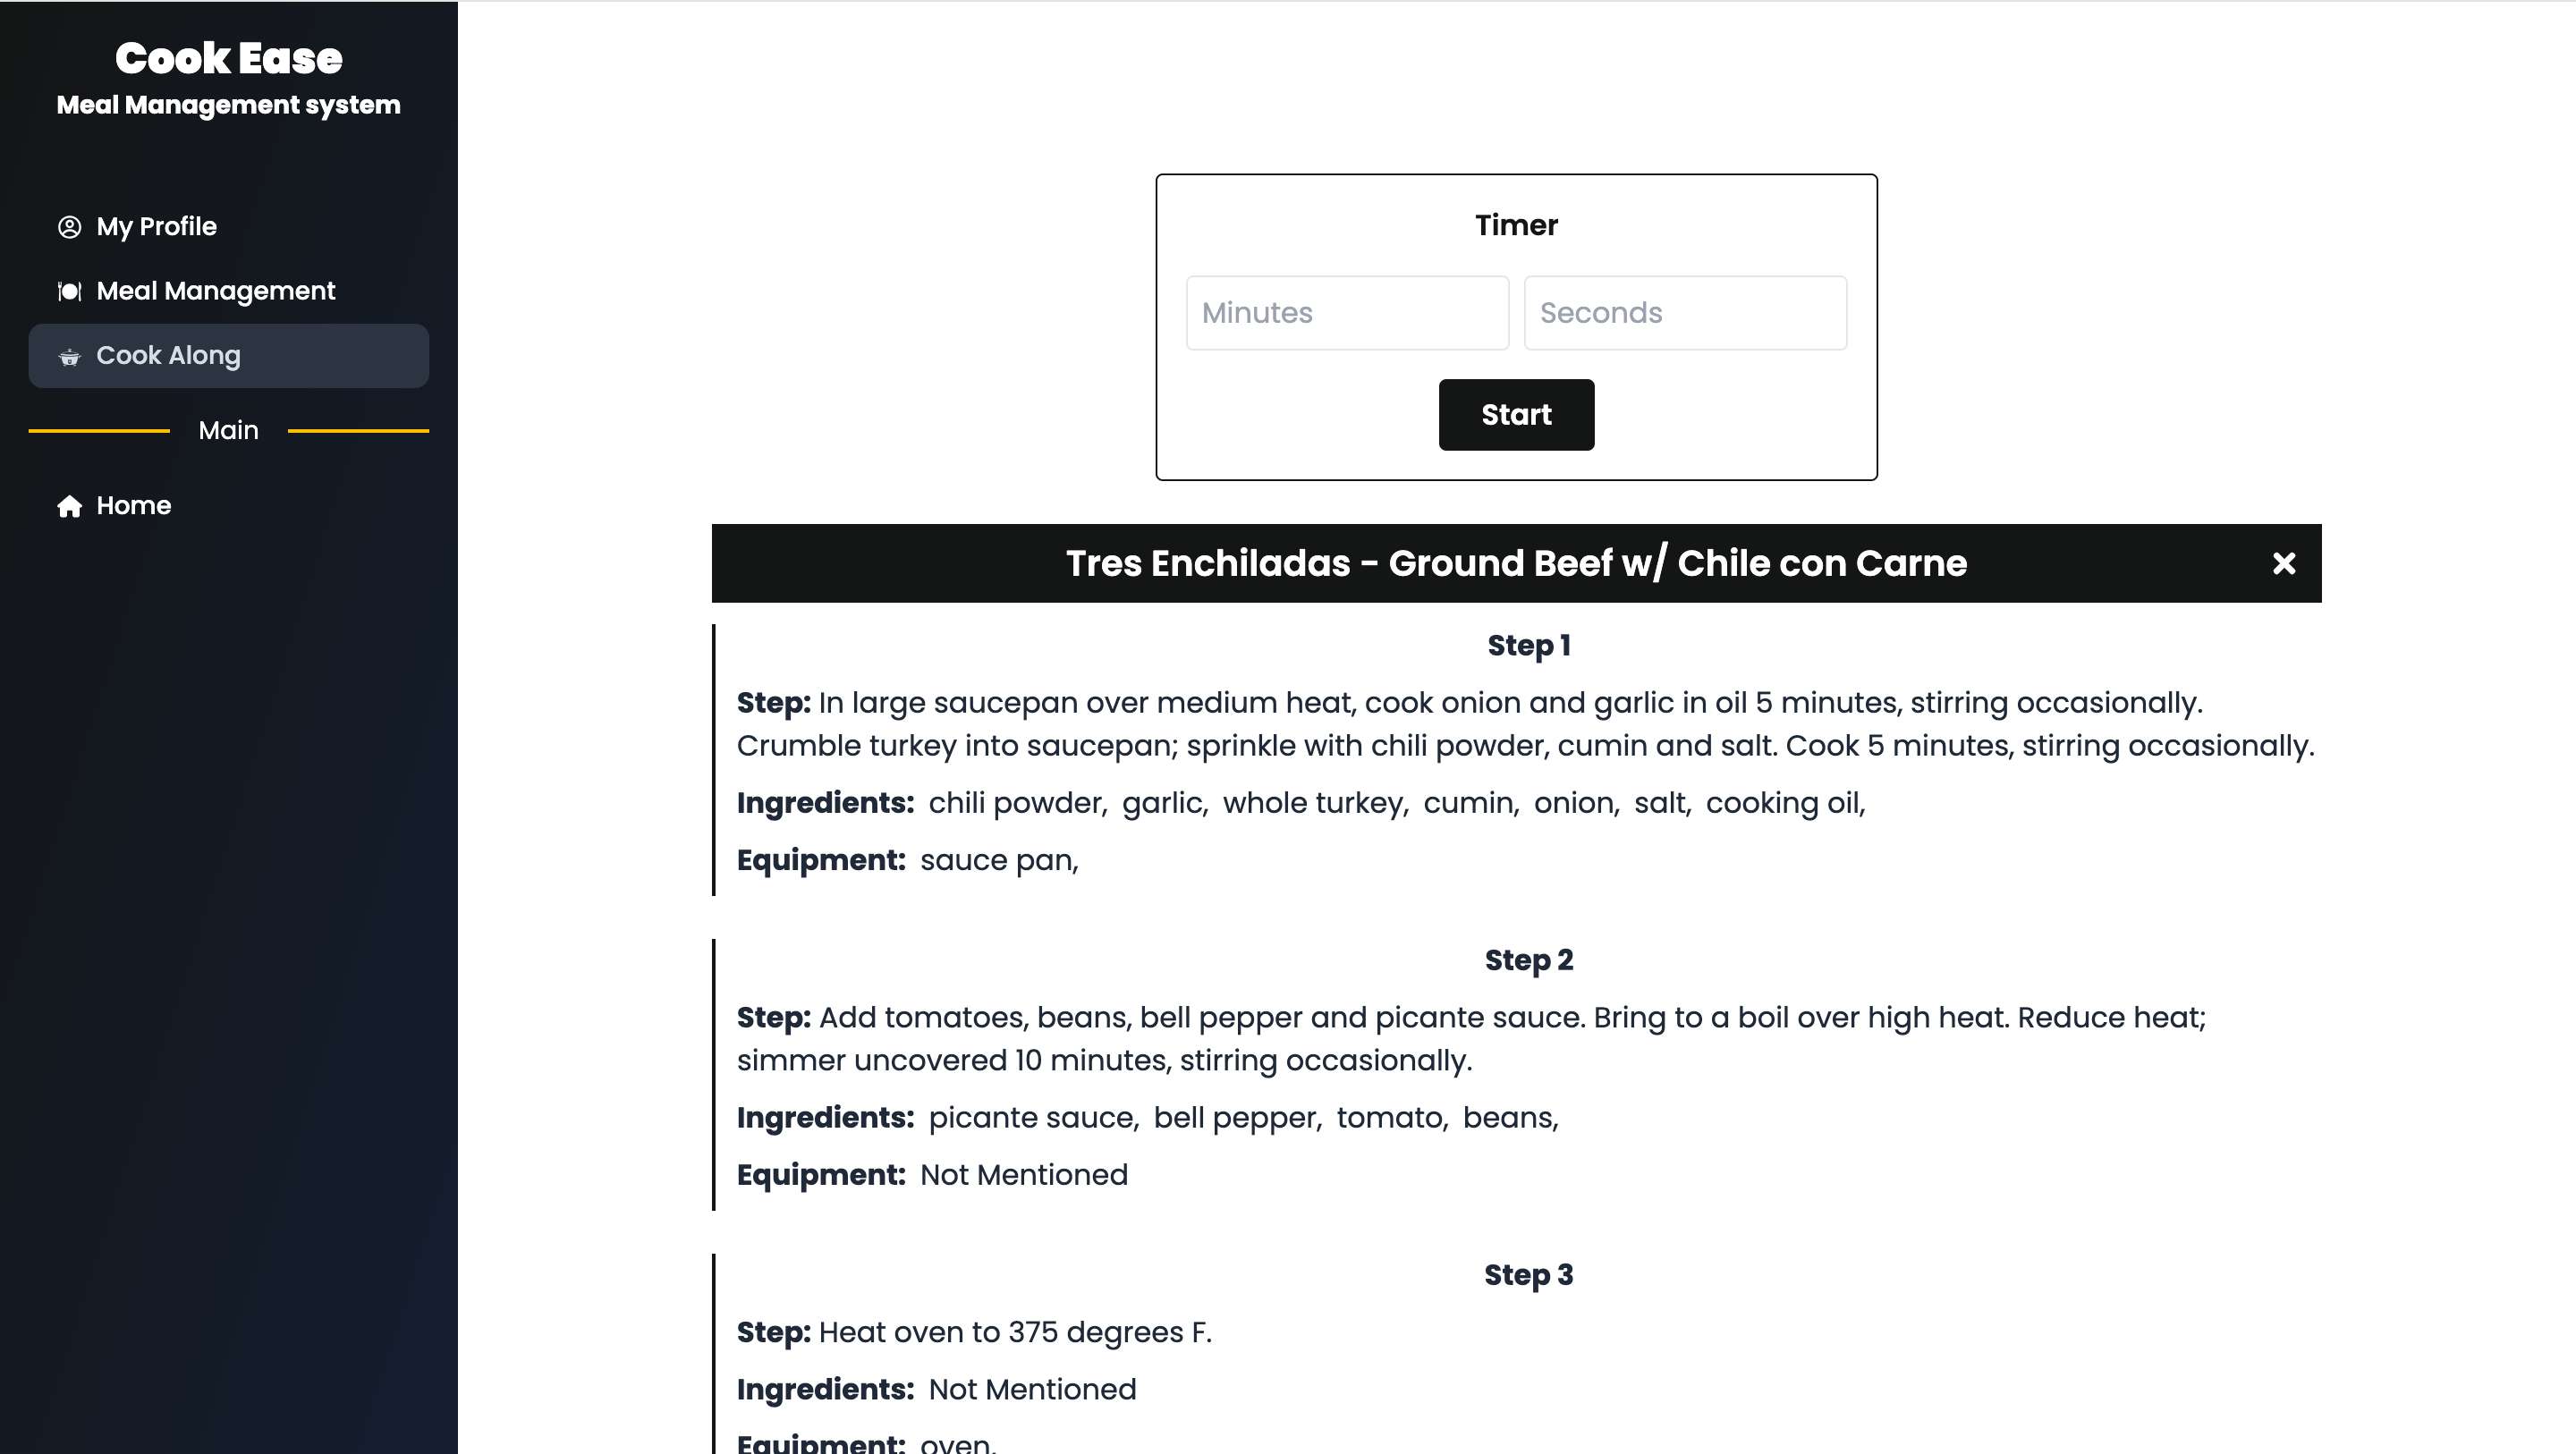
\includegraphics[width=0.5\textwidth]{images/Timer.png}
    \centering
    \end{figure} 
    
    \item Meal Planning: Users can create weekly meal plans using a simple search interface. The system links each meal to a recipe and provides an image and title of the recipe.
    \begin{figure}[h!]
    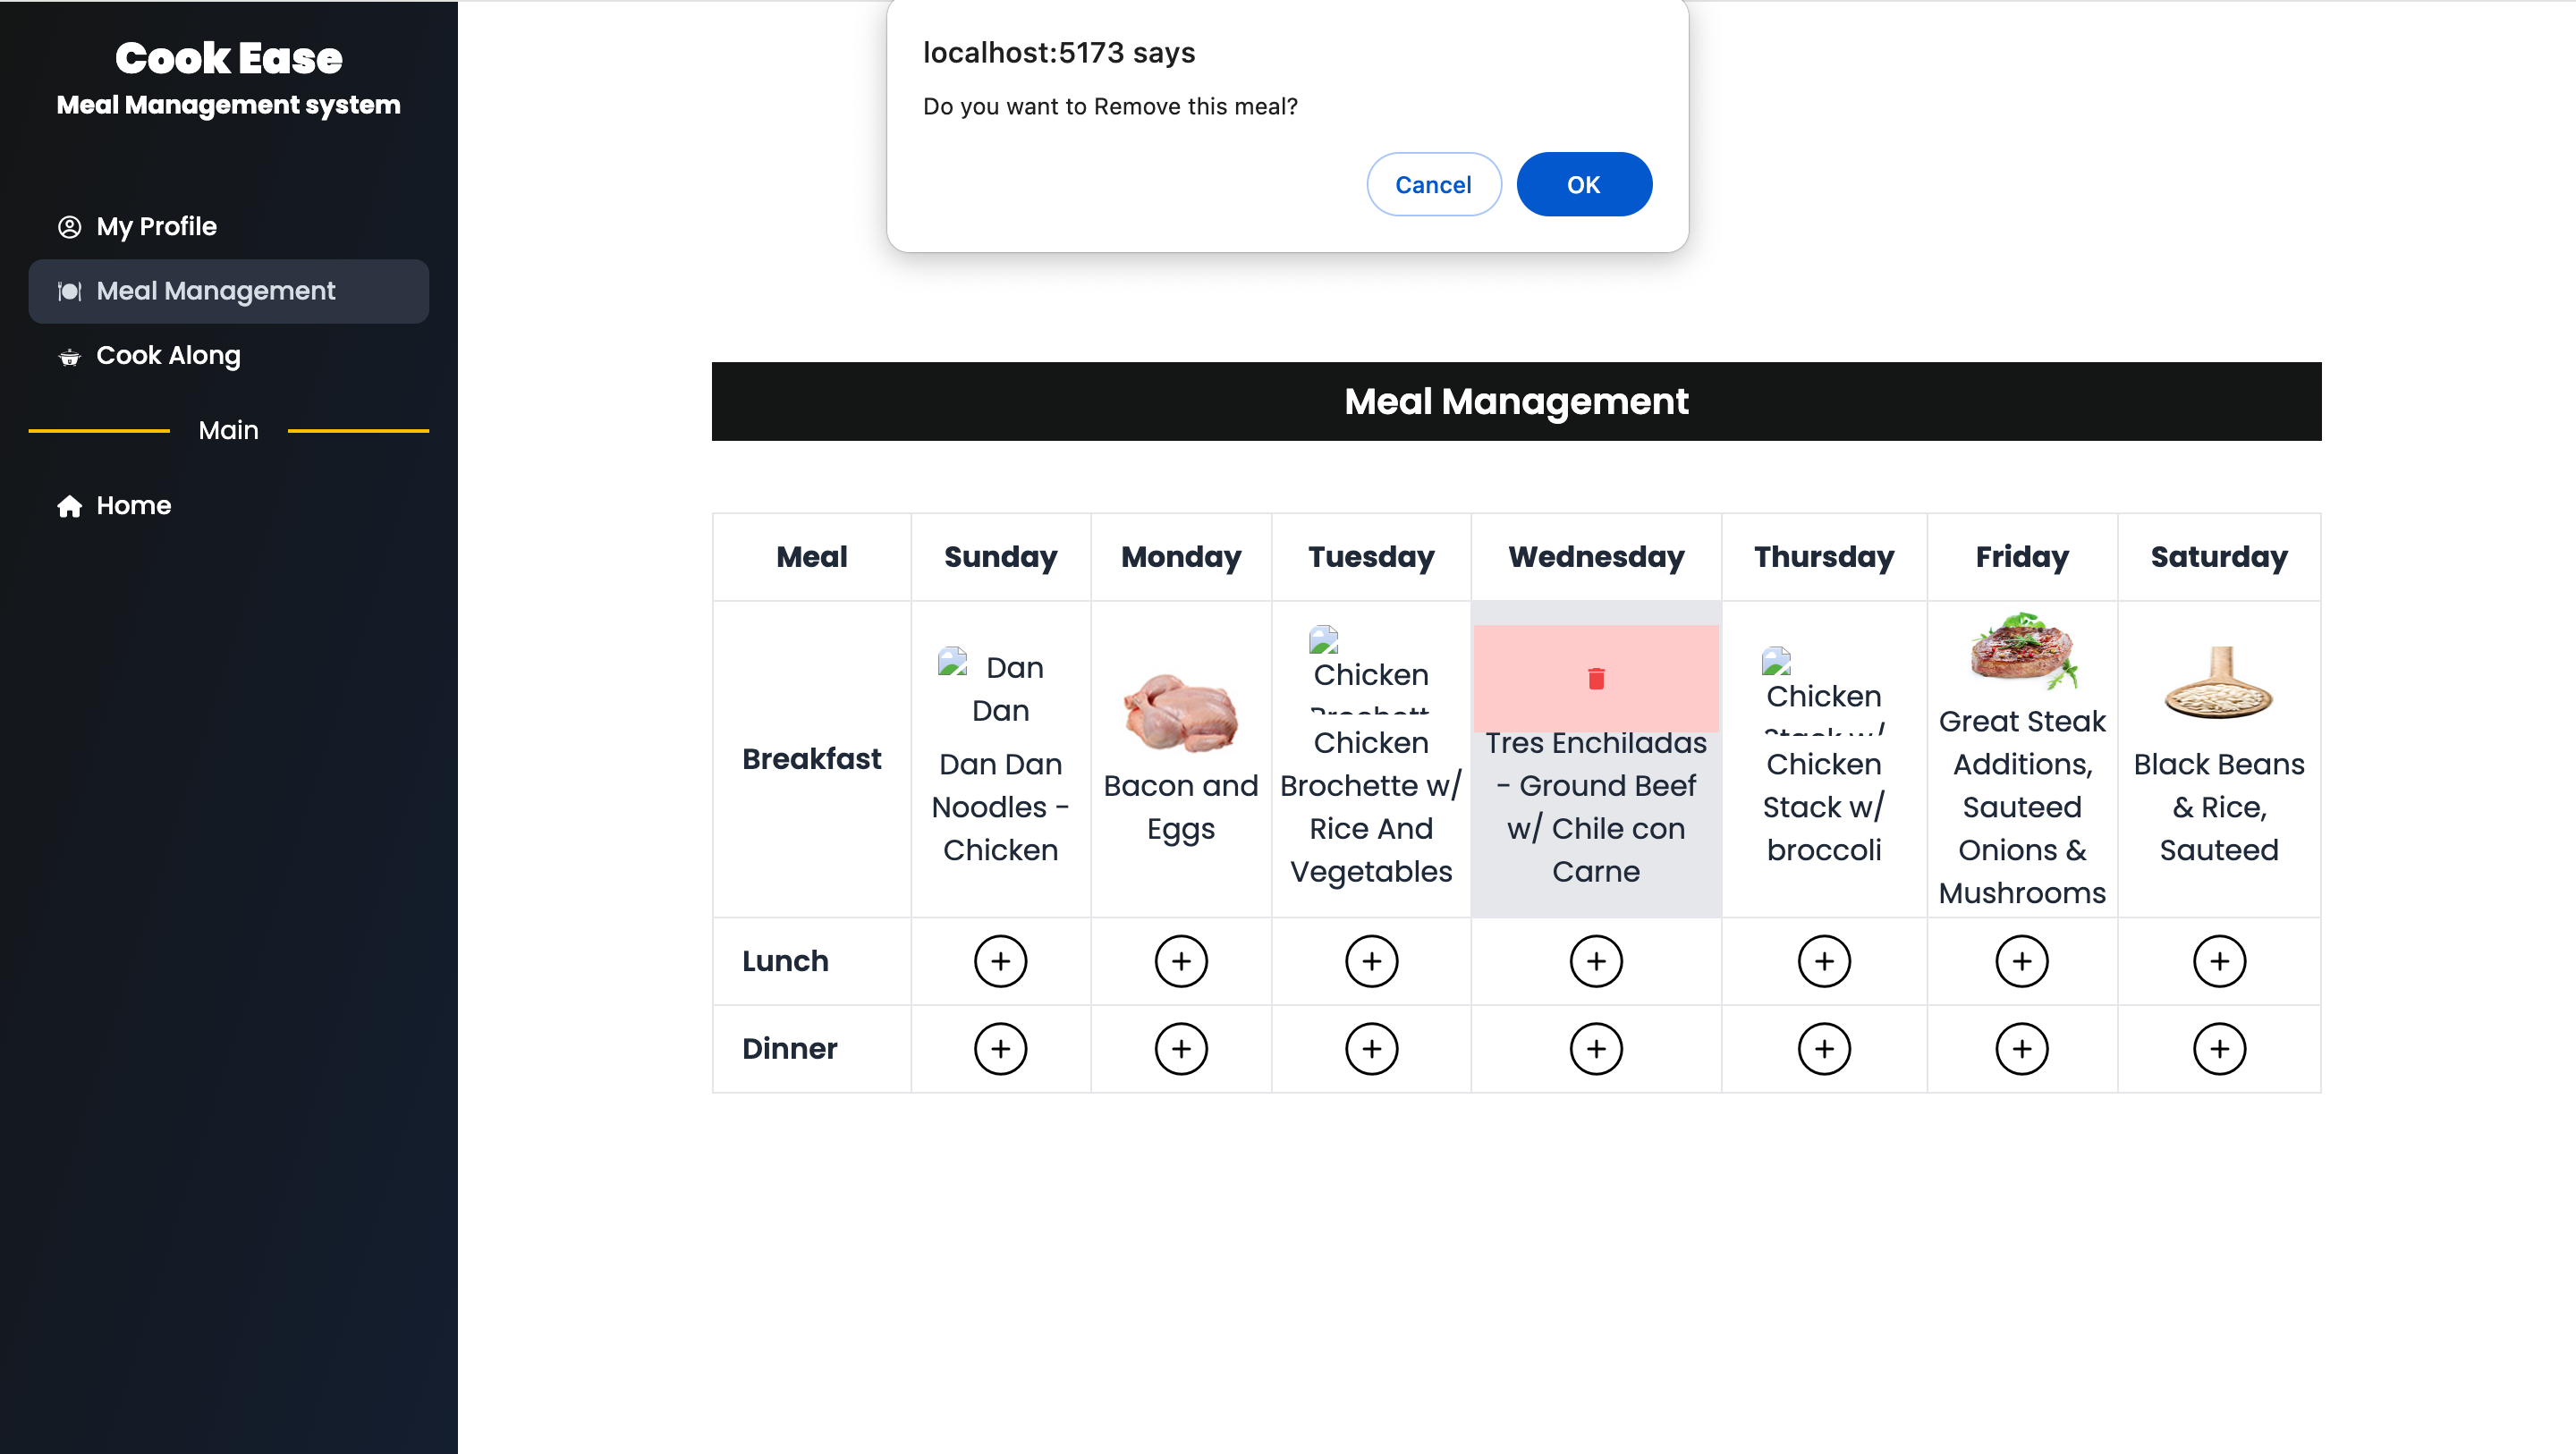
\includegraphics[width=0.5\textwidth]{images/MealPlan.png}
    \centering
    \end{figure} 
 
    \item Inventory Management: Users can manually update their inventory by adding or removing ingredients. The system provides reminders for items nearing expiration and highlights frequently used ingredients (In previous versions only). 
    \begin{figure}[h!]
    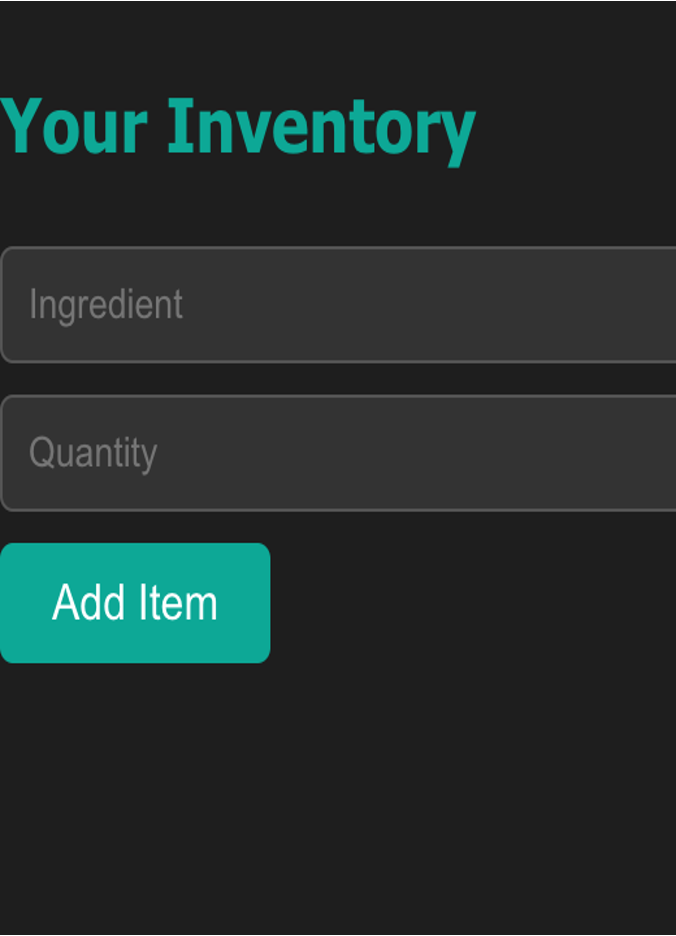
\includegraphics[width=0.5\textwidth]{images/OldInventory.png}
    \centering
    \end{figure} 
    \end{itemize}

\subsection{Justification of Design Choices}
Each design decision in CookEase is informed by user feedback and existing research. The modular structure of the MERN stack ensures scalability, allowing future features, such as barcode scanning for inventory updates (a feature brought up from multiple CS students), to be easily integrated. The reliance on the Spoonacular API leverages a robust dataset while reducing development overhead. Furthermore, the inclusion of interactive features like the Cook-Along guide directly addresses user-identified barriers, such as lack of confidence and cooking knowledge.

\section{Evaluation Metrics}
The evaluation of CookEase centers on assessing its impact on user confidence in cooking, alongside the usability and effectiveness of its key features. Confidence was chosen as the primary evaluation metric due to its significance for beginner cooks, who often face barriers such as intimidation by recipes, lack of experience, and disorganized meal planning. By evaluating how CookEase influences users’ confidence, this project aims to measure its success in addressing these barriers.

\subsection{Why Confidence is the Focus}
Cooking confidence is a critical factor that affects whether individuals engage with and sustain home cooking habits. Research has shown that building confidence through guided learning and structured support can encourage users to take more initiative in the kitchen\cite{Farmer2021}. Given CookEase's focus on providing clear instructions, personalized recipes, and structured meal planning, confidence is an appropriate and meaningful metric to evaluate its impact on users.

\subsection{Methods for Evaluating Confidence}
Confidence was evaluated through direct user testing, where participants interact with CookEase over a defined period (e.g., one week). During this period, I asked users to create weekly meal plans using the application, follow recipes through the Cook-Along guide, and provide feedback on their experiences. Data collection methods include:

Pre- and Post-Test Surveys: Participants will complete a survey before and after using CookEase to assess changes in their confidence. Questions include:
\begin{itemize}
    \item "How confident are you in planning meals for a week?" (Scale: 1-10)
    \item "How confident are you in following a recipe to completion?" (Scale: 1-10)
    \item "How confident are you in organizing your kitchen for cooking?" (Scale: 1-10)
\end{itemize}
Post-Use Interviews: Participants will be interviewed to gain qualitative (constructive feedback) and quantitative (user engagement) insights into how CookEase influenced their confidence and what aspects of the application contributed to or hindered it.

\subsection{Expected Outcomes}
Based on the design and objectives of CookEase, the following outcomes are anticipated:

Increased Confidence Scores: Users should report higher confidence scores post-trial, particularly in areas related to meal planning and recipe execution.
High Engagement with Features: Features like the Cook-Along guide and meal planning tool are expected to show consistent use, indicating their effectiveness in reducing barriers for beginner cooks.
Constructive Feedback for Improvement: Users are likely to identify areas where the application could better support their needs, such as bug fixes or feature enhancements.

\section{Results and Discussion}
The evaluation of CookEase focuses on assessing user confidence in cooking, and qualitative feedback to understand the strengths and limitations of the application. The following section explores the results obtained through user testing and discusses the implications for CookEase's future development.

\subsection{Confidence Levels}
The primary metric of success for CookEase was its ability to improve user confidence in cooking. Using pre- and post-test surveys, users were asked to rate their confidence in meal planning, recipe following, and kitchen organization on a scale of 1 to 10 before and after a week of using CookEase.

Pre-test results showed average scores of 5 for meal planning confidence, 4 for recipe following confidence, and 3 for kitchen organization confidence.
Post-test results revealed significant improvement, with average scores increasing to 8 for meal planning confidence, 7 for recipe following confidence, and 6 for kitchen organization confidence.
\begin{figure}[h!]
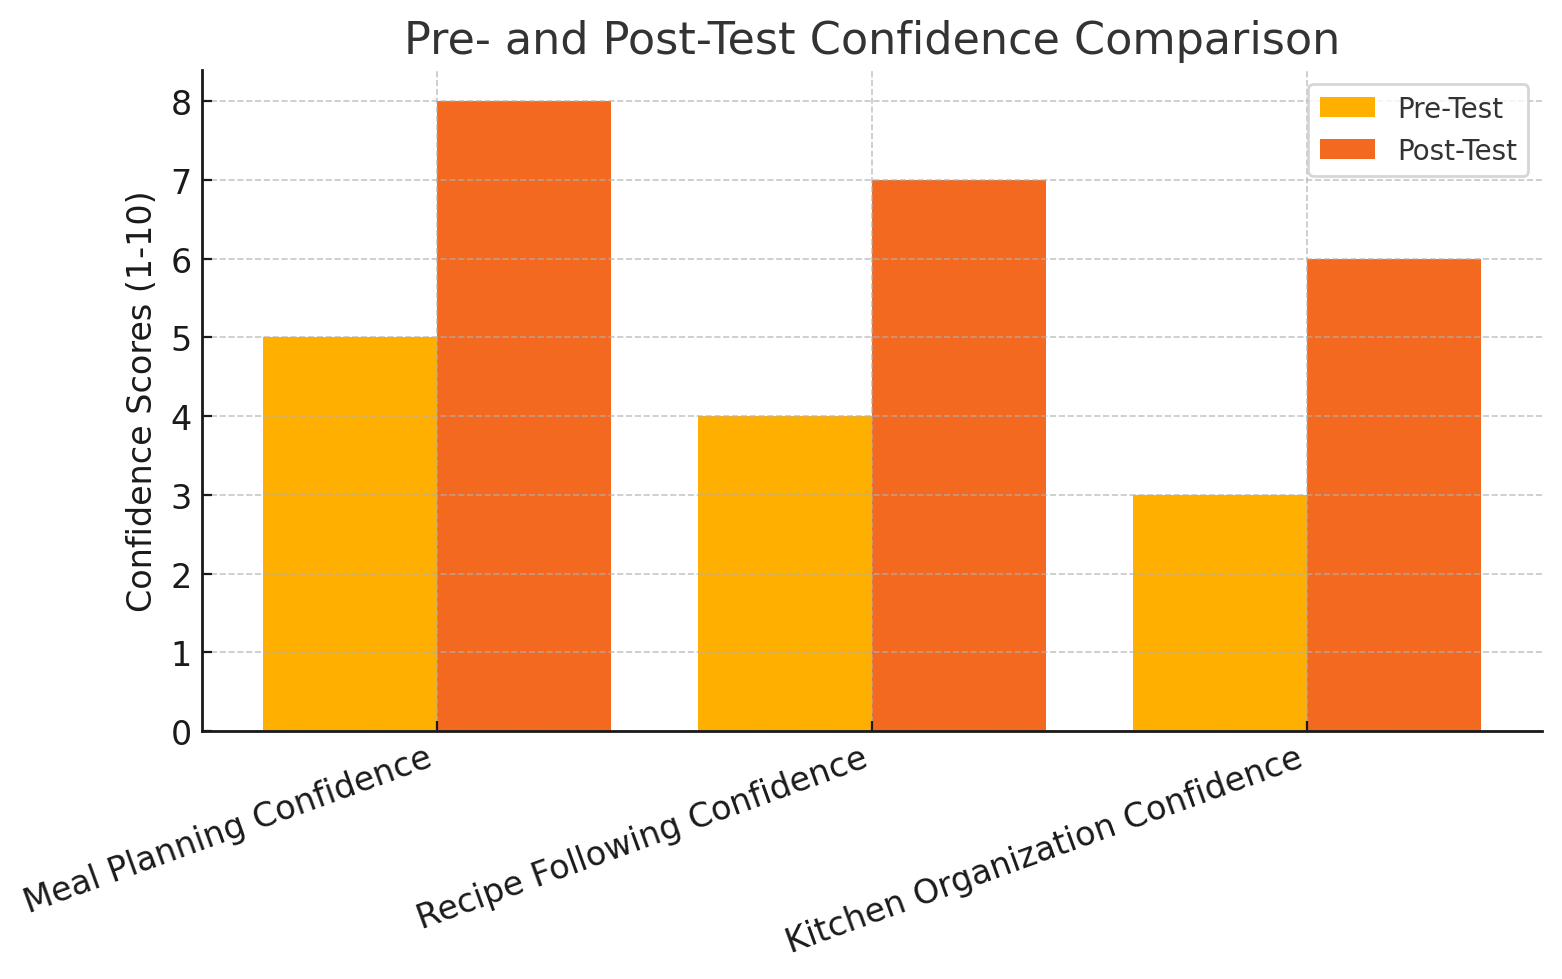
\includegraphics[width=0.5\textwidth]{images/pre-postconfidence.png}
\centering
\end{figure} 
This substantial increase in confidence levels demonstrates CookEase's potential to address critical barriers for beginner cooks. However, some variability in results was observed, as certain users noted frustrations with incomplete features, such as occasional bugs in the Cook-Along component where incorrect meals would be displayed.

\subsection{Qualitative Feedback}
User feedback provided deeper insights into the strengths and weaknesses of CookEase:
\subsubsection{Areas for Improvement:}
Bugs in the Cook-Along feature, such as incorrect recipe steps, detracted from user experience.
Users suggested integrating the inventory feature into a dedicated user profile page to streamline its use and enhance recipe recommendations (under development).
\begin{figure}[h!]
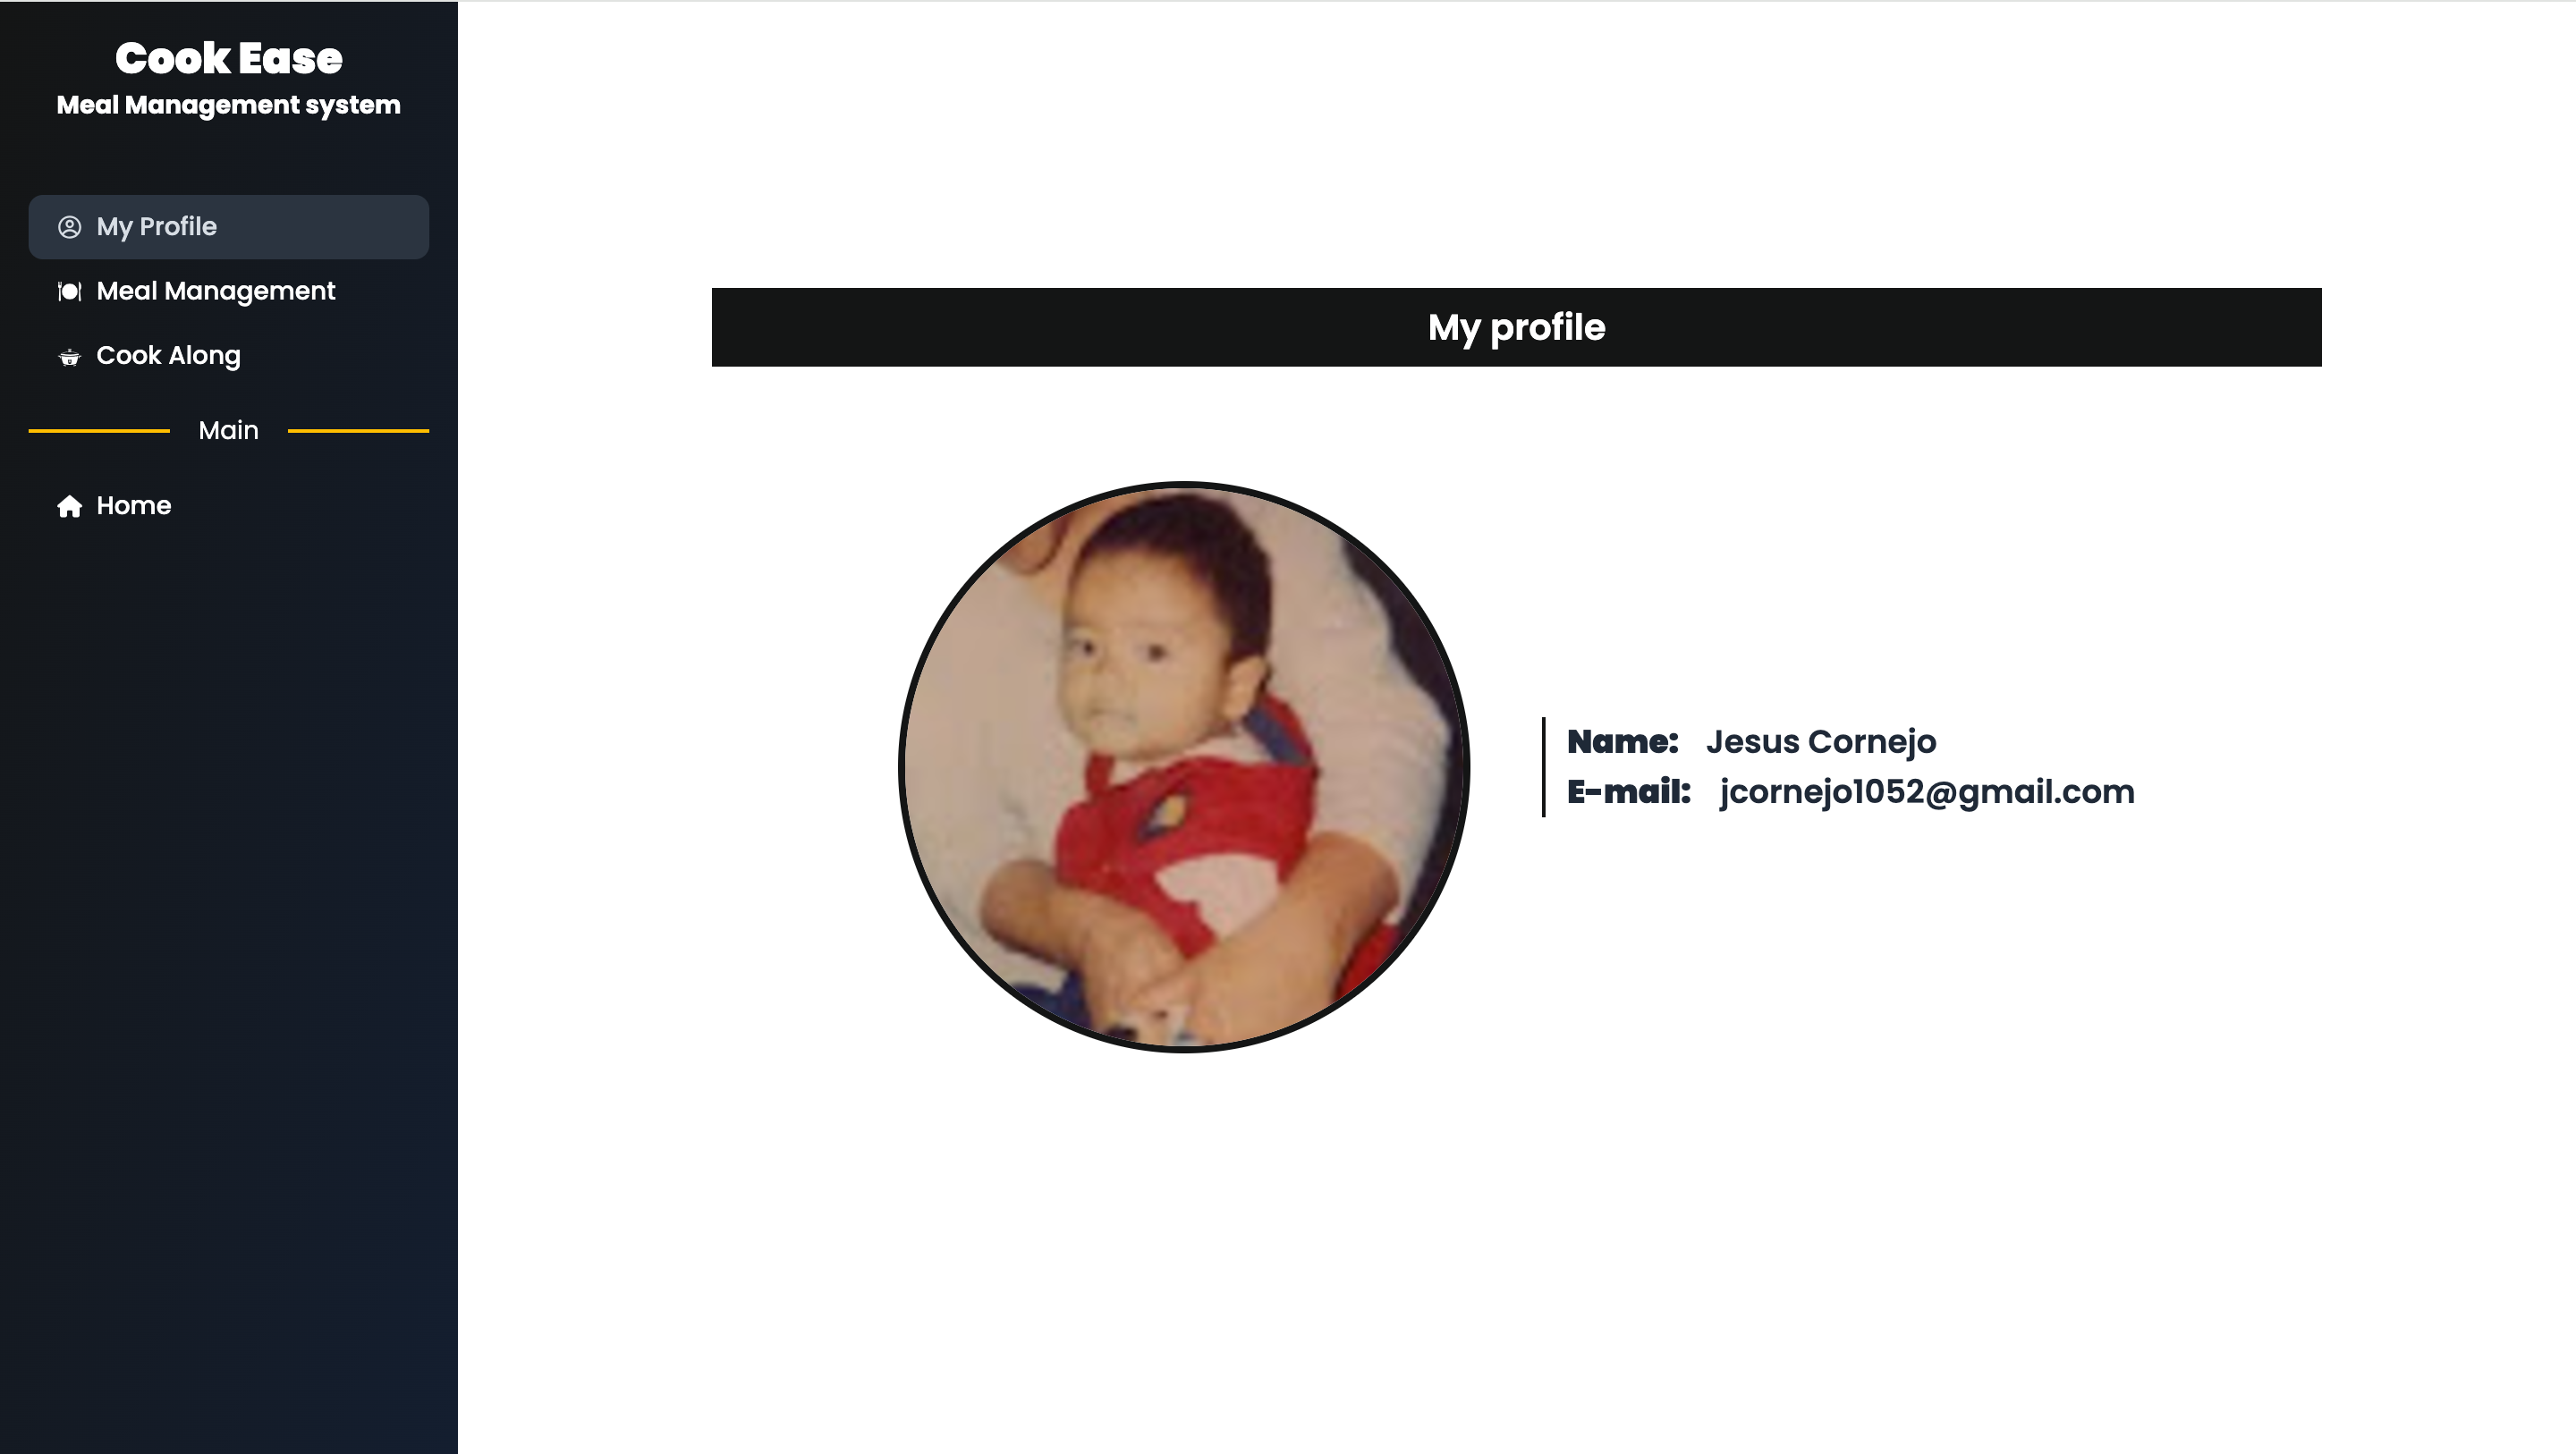
\includegraphics[width=0.5\textwidth]{images/UserProfile.png}
\centering
\end{figure} 
The absence of reminders for meal plans was noted as a missed opportunity to improve organization (under development).
\begin{figure}[h!]
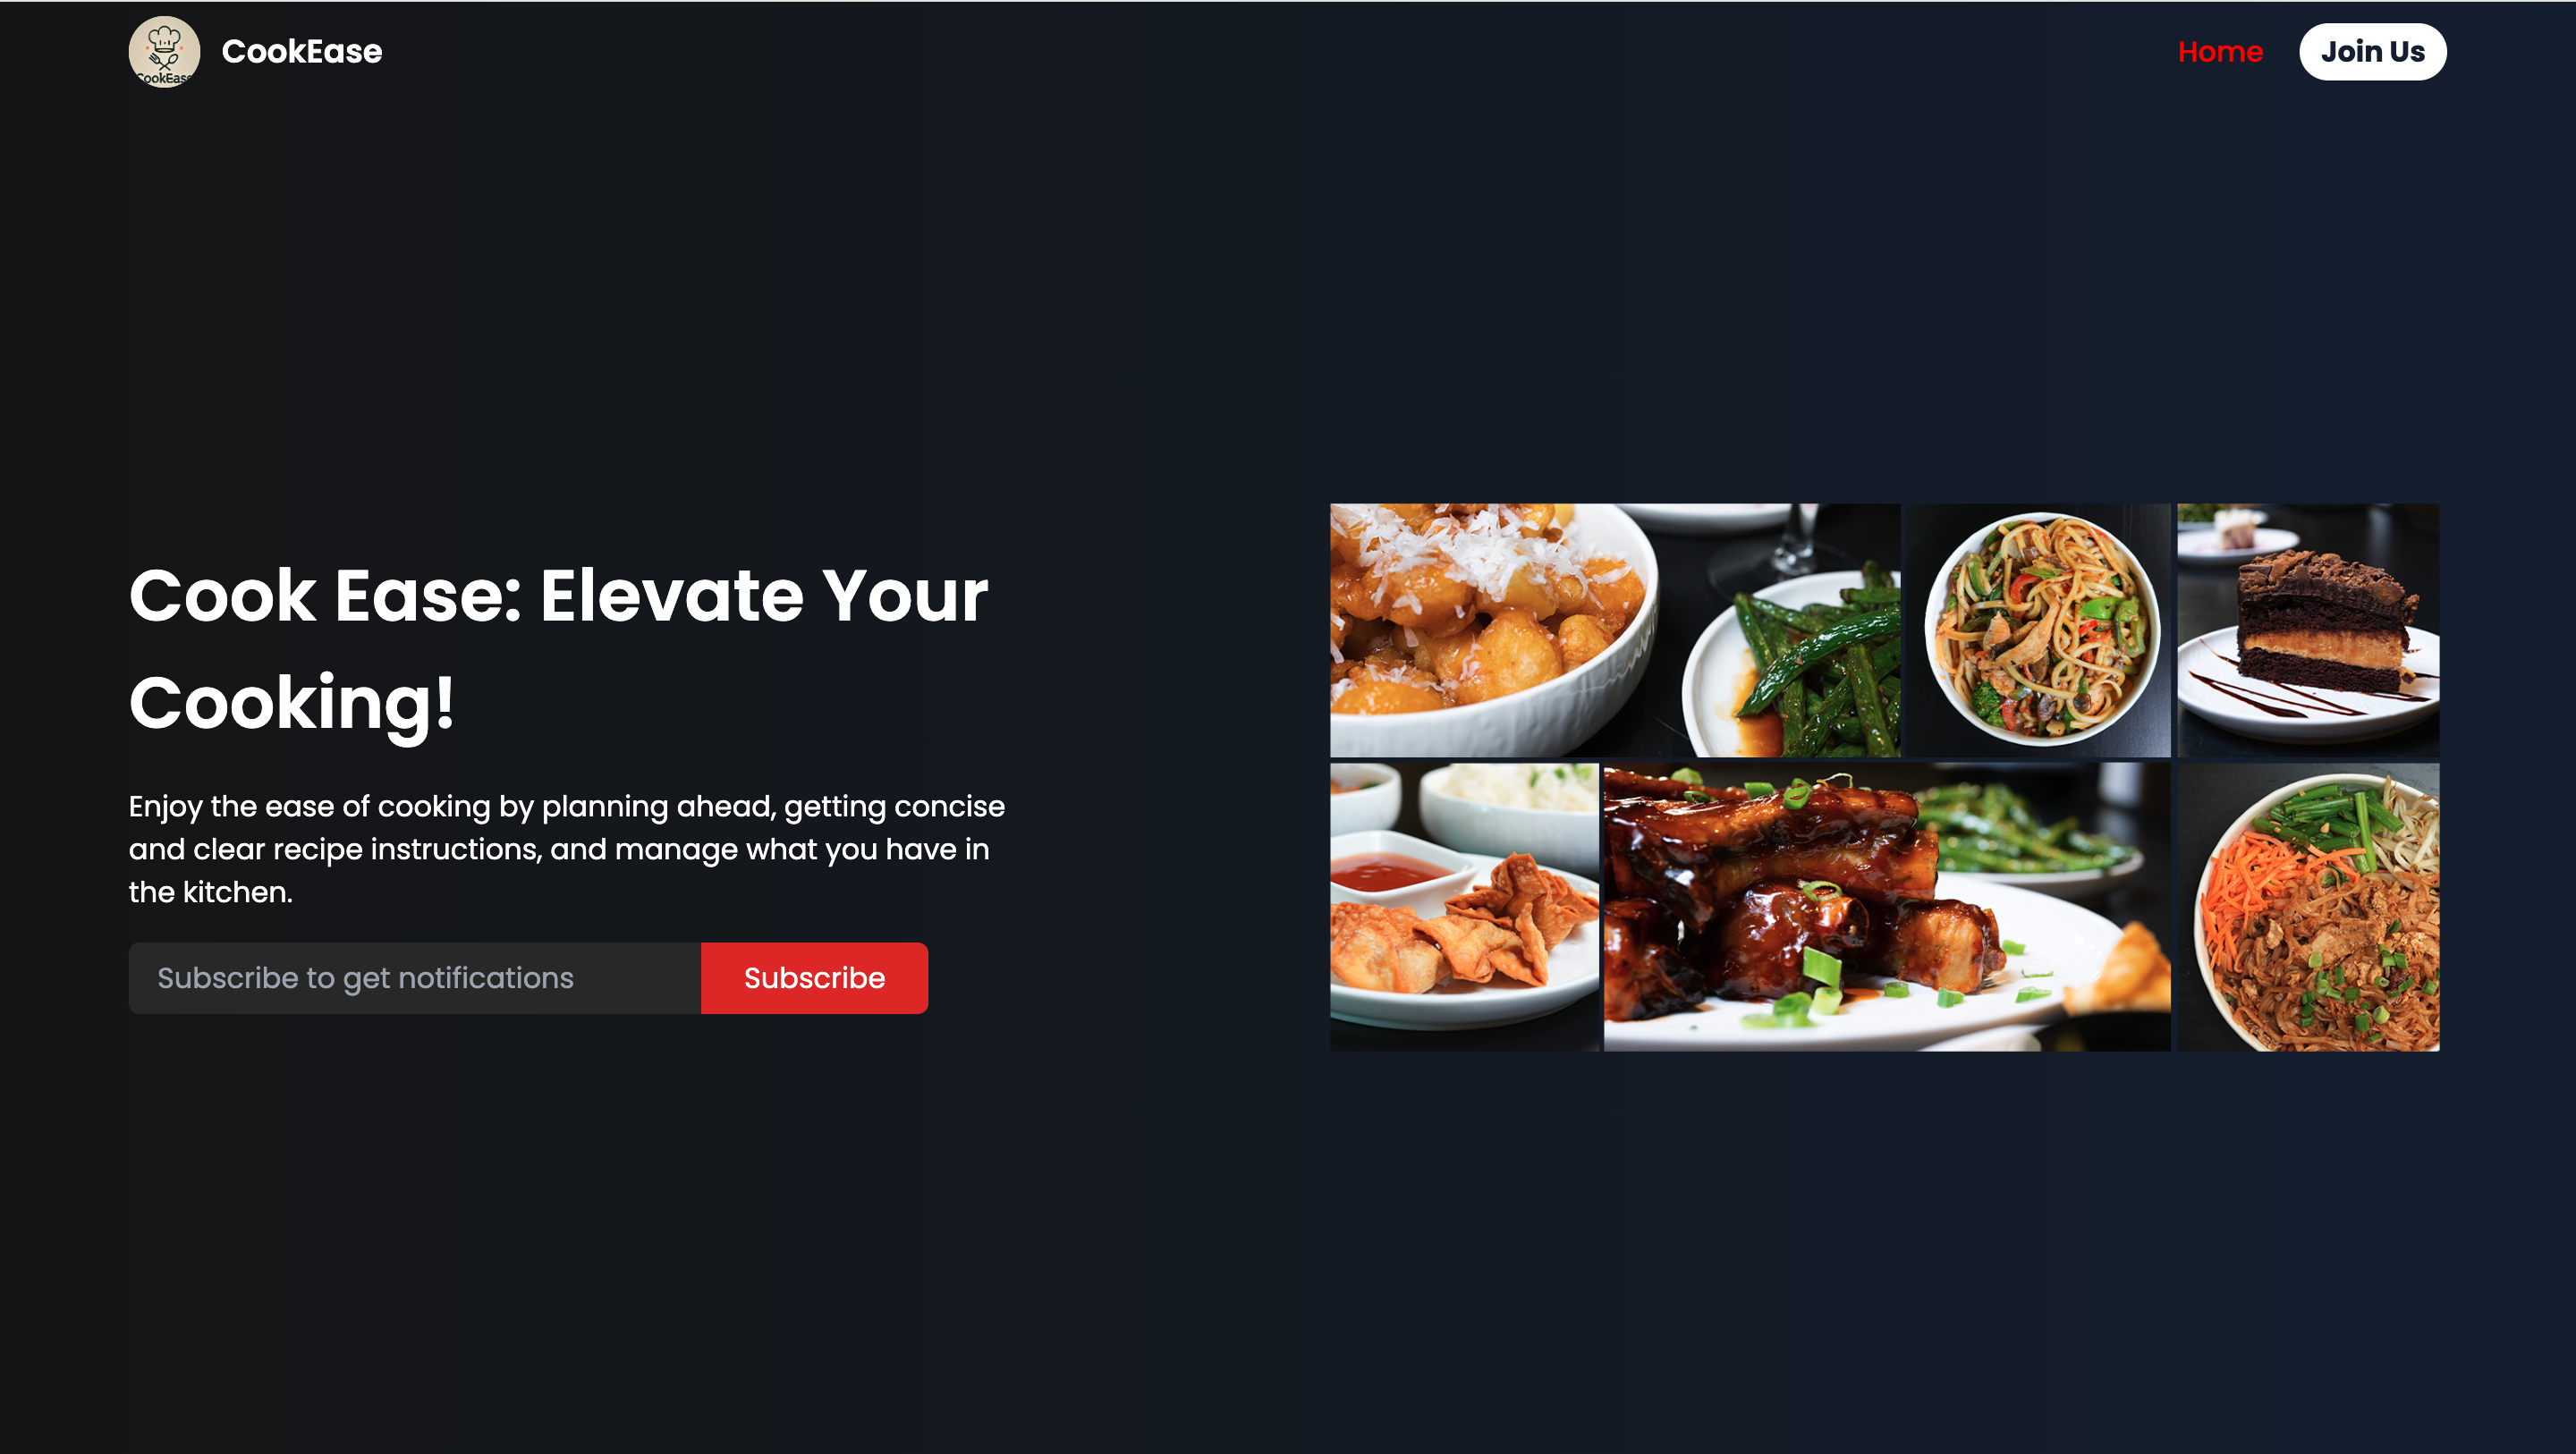
\includegraphics[width=0.5\textwidth]{images/JoinUS.png}
\centering
\end{figure} 

\subsection{Discussion}
The results of user testing demonstrate that CookEase has significant potential as a tool for beginner cooks but also highlight critical areas for refinement. The marked improvement in confidence scores indicates that the application effectively addresses some common barriers to cooking, such as planning and following recipes. However, the variability in qualitative feedback underscores the need for a more polished and reliable user experience.

The high engagement with the Cook-Along feature shows its value as a core component of CookEase. However, bugs and incomplete functionalities reduce its effectiveness. Addressing these issues through rigorous testing and refinement will be essential to fully realize its potential.

The feedback on meal planning and inventory integration reveals opportunities to streamline the user experience further. Incorporating dietary preferences and inventory tracking into a centralized user profile could enhance personalization and simplify recipe recommendations. Additionally, adding reminders to the meal-planning feature could improve its usability and encourage consistent use.

\subsubsection{Next Steps}
The insights gained from this evaluation suggest several priorities for the next phase of CookEase development:

Fixing bugs and improving the reliability of the Cook-Along feature to enhance user satisfaction.
Reorganizing the interface to better integrate inventory tracking, dietary preferences, and user profiles.
Adding notifications and reminders for meal plans to support user organization and consistency.
Expanding user testing to a larger and more diverse audience to validate improvements and refine the application. Because of time limitations a wide enough population of user testing was not available, but additionally Spoonacular API sets quotas (limit) on the amount of requests made.
Implementing User Logs: The application will track user interactions, such as the number of meal plans created, recipes viewed, and steps completed in the Cook-Along guide. These metrics will provide indirect indicators of user engagement and potential confidence growth.
By addressing these areas, CookEase can evolve into a more comprehensive and user-friendly platform, better aligned with its mission to empower beginner cooks and make cooking a more enjoyable and accessible experience.

\section{Ethical Considerations}
The CookEase project aims to promote sustainable cooking habits and empower beginner cooks by providing accessible tools for meal planning and recipe guidance. However, several ethical considerations must be addressed to ensure that the application does not perpetuate societal inequities or introduce unintended consequences.
\begin{itemize}
    \item Bias in Recipe and Dietary Recommendations: 
    The Spoonacular API and user-generated inputs may inadvertently reflect biases in cultural representation or dietary preferences. To mitigate this, CookEase will strive to provide diverse and inclusive recipe suggestions by prioritizing a wide range of cuisines and ensuring that the algorithm does not unfairly rank certain cuisines higher than others without user preference.
    \item Data Privacy and Security:
    CookEase collects sensitive user data, such as dietary preferences, kitchen inventory, and meal schedules. Ensuring that this data is stored securely and used only for its intended purpose is a top priority. The application employs industry-standard encryption for data storage and transmission (through firebase authentication), and user consent is required for any data collection. Additionally, data anonymization techniques will be considered for analytics to further safeguard user privacy.
    \item Access to Technology: 
    As a web-based application, CookEase relies on users having access to the internet and modern devices. This could exclude individuals in low-income communities or areas with limited internet connectivity. Future development efforts should explore offline functionality or partnerships with organizations to provide broader access to digital tools for cooking education.
\end{itemize}

\section{Appendices}
\appendix
\section{Replication Instructions}
To replicate the CookEase application, follow these steps:

1. Prerequisites
Ensure you have the following tools installed on your development environment:

Node.js (v14 or higher)
MongoDB (running locally or hosted)
NPM or Yarn (for package management)
2. Project Setup
Download and Extract:

Download the CookEase project files and extract them to a local directory.
Install Dependencies:

Navigate to the root directory of the project.
Run npm install in both the client and server directories to install required dependencies.
Set Up Environment Variables:

In the server directory, create a .env file with the following:
\begin{itemize}
    \item MONGO\_URI=your\_mongo\_database\_uri
    \item SPOONACULAR\_API\_KEY=your\_spoonacular\_api\_key
    \item PORT=5000
\end{itemize}

In the client directory, create a .env.local file if needed to store any client-specific environment variables.

Start MongoDB:
Ensure MongoDB is running locally or provide the URI for a hosted MongoDB instance in the .env file.

Run the Application:
In the server directory, run npm start to start the backend server.
In the client directory, run npm run dev (if using Vite) to start the frontend.

Access the Application:
Open your browser and navigate to http://localhost:3000 to interact with the CookEase application.
\subsection{Data Flow Overview}
The CookEase system architecture is designed as follows:

Frontend (React):
Gathers user input (inventory, preferences, and actions).
Displays data (recipes, schedules, Cook-Along guides).
Backend (Express):
Processes requests from the frontend.
Handles database operations and API requests to Spoonacular.
Database (MongoDB):
Stores user data, including inventory, preferences, and meal plans.
Spoonacular API:
Provides recipe recommendations based on user input.
\textbf{include diagram from poster pres}

\section{Code Overview}

\subsection{Server Directory}
The server-side implementation of CookEase is built using Node.js and Express.js, providing a robust backend framework for managing API requests, database operations, and user authentication. The index.js file serves as the entry point, setting up the Express app, connecting to MongoDB using Mongoose, and defining middleware for parsing JSON, handling CORS, and logging requests. It also integrates API routes for user authentication, recipe generation, inventory management, and meal planning. Environment variables, such as the MongoDB connection URI, Spoonacular API key, and server port, are stored in the .env file for secure and flexible configuration.

Core functionalities include API routing and database modeling. API routing handles user authentication, retrieves recipe recommendations by interacting with the Spoonacular API, and manages user inventory and meal plans. Database models define the structure for user data, recipes, and meal plans. The User model stores details like username, email, dietary preferences, and kitchen inventory. The Recipe model contains recipe metadata, including ingredients, steps, and nutritional information. The MealPlan model organizes scheduled recipes, linking them to specific dates and times.

\subsection{Client Directory}
The client-side of CookEase, developed using React, provides a dynamic and user-friendly interface. The application's structure is modular, ensuring maintainability and scalability. The entry point, main.jsx, initializes the React app and integrates routing via React Router. The main application logic resides in App.jsx, which manages global state and renders core features like inventory management, meal planning, and the Cook-Along guide. Styles are defined in index.css, ensuring a consistent design across components.

The src directory contains several subdirectories, each serving a specific purpose. The Providers directory includes AuthProvider.jsx for managing user authentication context and firebase.config.js for potential Firebase integration. The Components directory houses reusable UI elements, such as NavBar.jsx for navigation, HomeBanner.jsx for the homepage, and specialized tools like Meal.jsx and Timer.jsx for the dashboard. Shared components like ErrorPage.jsx and Loader.jsx enhance usability and provide fallback mechanisms for errors or loading states.

The Layouts directory structures pages, such as Dashboard.jsx for managing features and a user-specific subdirectory with components like CookAlong.jsx for step-by-step recipe guidance, MealManagement.jsx for meal plan editing, and MyProfile.jsx for user details. The Hooks directory offers custom hooks like useAxiosPublic.jsx for public API requests, useAxiosSecure.jsx for authenticated requests, and useUser.jsx for managing user-specific data.

Page-specific components, located in the Pages directory, include HomePage.jsx, LoginPage.jsx, RegistrationPage.jsx, and DetailsPage.jsx, each rendering distinct sections of the application. The Routes directory manages navigation and access control with Routes.jsx defining general navigation and UserRoute.jsx restricting routes to authenticated users.

\printbibliography

\end{document}
